\chapter{拥塞感知初始布线工作流}
\label{cha:congestion-aware-initial-routing}

\section{本章引言与问题定义}
\label{sec:chap3-intro}

第二章从后端设计流程与全局布线技术基础出发，给出了树生成、模板布线、层分配与迷宫布线的标准流程。结合第一章的问题陈述可知，在先进工艺节点和超大规模设计背景下，全局布线面临两个同时存在且互相制约的核心矛盾：一是前期决策质量不足导致拥塞在流程中后期集中爆发，二是串行或弱并行流程难以支撑超大规模线网的计算吞吐需求。

在传统工作流中，在全局布线的第一阶段为树生成阶段，此阶段通常采用FLUTE算法生成树拓扑，因此传统算法中通常以线长最优为主导，较少考虑拥塞信息，导致前期候选解空间偏窄。当模板布线阶段再叠加有限模板搜索时，这种偏差会进一步放大，最终将大量高难度线网推入撤销重布（Rip-up and Reroute）与迷宫布线阶段，造成运行时间显著上升，并使后期修复空间受到限制。针对该问题，本文将研究重点前移到初始布线阶段，构建可感知拥塞、可迭代更新、可并行求解的初始布线工作流。

本章所述方法聚焦于动态拥塞感知初始布线工作流，本文在该方向上的直接贡献可归纳为三点：
\begin{enumerate}
    \item 提出拥塞感知的候选树森林构建机制，在初始化阶段同时保留线长导向与拥塞感知导向两类树拓扑，为后续联合优化提供更有区分度的候选空间；
    \item 将面向并行平台的求解流程集成在此初始布线工作流中，将数据级并行与线网级并行协同嵌入初始布线求解过程，在控制质量退化风险的前提下提升整体效率。
    \item 提出动态更新树森林与迭代剪枝树森林机制，在多轮训练之间分别处理拥塞线网与非拥塞线网，使优化资源持续聚焦于真正的瓶颈区域；
\end{enumerate}

围绕上述目标，本章组织如下：第\ref{sec:chap3-framework}节给出总体流程；第\ref{sec:chap3-forest}节讨论候选树森林构建；第\ref{sec:chap3-diff-model}节给出可微解析建模；第\ref{sec:chap3-dynamic}节给出拥塞初始布线动态工作流构建方法；第\ref{sec:chap3-engineering}节给出工程实现细节；第\ref{sec:chap3-parallel}节给出并行层次分析；第\ref{sec:chap3-exp}节给出实验设置与结果分析；第\ref{sec:chap3-summary}节给出本章小结。

\section{动态拥塞感知初始布线总体框架}
\label{sec:chap3-framework}

\subsection{工作流总体思路}

本文采用拥塞感知初始树森林构建、可微建模、动态更新树森林、动态缩减树森林等策略，并进行迭代收敛。与单轮训练的静态流程相比，该闭环机制在每一轮结束后主动重构后续轮次的候选空间，使初始布线变成动态的优化过程。

具体而言，给定线网集合 $\mathcal{N}$ 与全局网格资源图，首先为每个线网构建由两个候选树拓扑组成的树森林：其一是由FLUTE生成的直角斯坦纳最小树（Rectilinear Steiner Minimum Tree, RSMT）\cite{10.1109/TCAD.2007.907068}，其二是基于当前拥塞信息生成的绕线树。随后，在树森林及其对应的两引脚模板候选上建立两层概率变量，通过可微目标函数联合建模线长、通孔与拥塞溢出代价，使用并行优化器（如基于PyTorch的Adam或SGD梯度下降优化器）进行多轮迭代求解。每轮求解后，对仍拥塞线网执行动态更新树，对已无拥塞线网执行动态缩减，从而进入下一轮训练。整体流程如图\ref{fig:chap3-overall-flow-placeholder}所示。


\begin{figure}[!htbp]
    \centering
    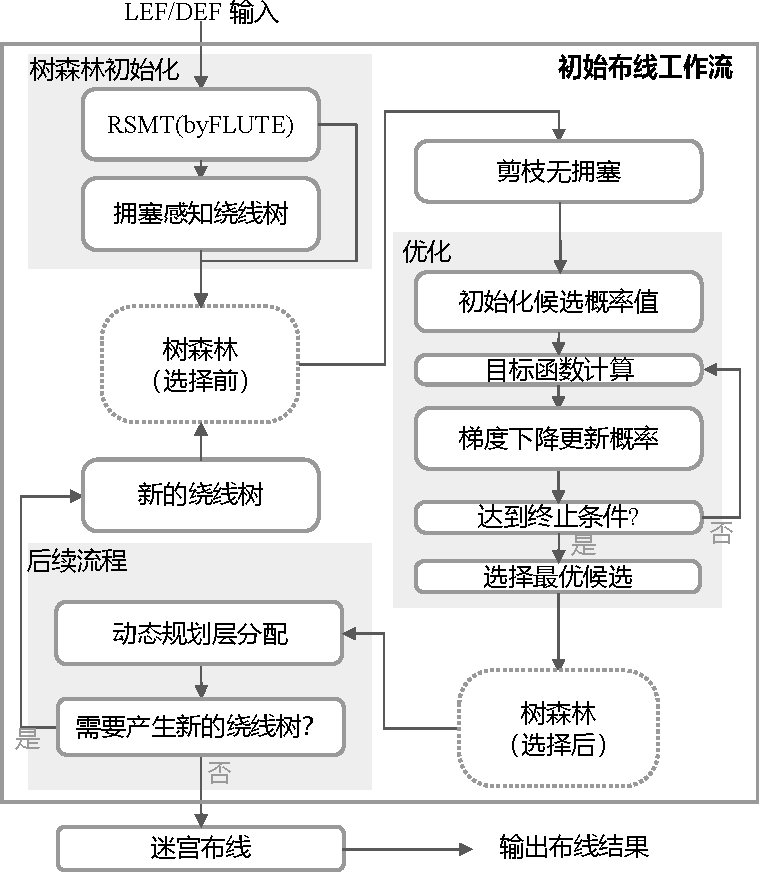
\includegraphics[width=0.95\textwidth]{image/chap03/初始布线工作流程图.pdf}
    \caption{动态拥塞感知初始布线总体流程}
    \label{fig:chap3-overall-flow-placeholder}
\end{figure}

\subsection{与基线流程的差异化设计}

与DGR\cite{10.1145/3649329.3656530}等可微全局布线方法相比，本文流程的差异主要体现在两个方面。

第一，树森林初始化更强调拥塞信息前置。传统做法常在后期修复阶段处理拥塞，而本文在初始构建时就将绕拥塞能力纳入候选拓扑，使早期解空间具备更强可塑性。

第二，训练轮次之间引入结构化反馈。DGR工作中仅执行单次的模板布线，优化效果存在一定的局限。本文对其算法进行拓展，构建动态更新树森林的循环布线工作流，充分发挥并行算法的优化潜力。


\section{候选树森林构建机制}
\label{sec:chap3-forest}

\subsection{树森林数据结构与层次关系}

本文将全局初始布线的候选空间组织为树森林（Tree Forest）结构。对于每个线网 $n \in \mathcal{N}$，定义其候选树集合为 $\mathcal{T}_n=\{t_n^{(1)}, t_n^{(2)}\}$，其中 $t_n^{(1)}$ 为RSMT候选，$t_n^{(2)}$ 为拥塞感知绕线树候选。每棵树进一步分解为若干两引脚边 $e$，每条两引脚边对应某个模板路径候选 $\mathcal{P}_{n,e}$。

该结构具有两层决策：第一层为树拓扑层次选择，第二层为树内两引脚路径选择。两层联合决定最终初始布线方案。通过该分层表达，离散组合优化问题可在后续建模阶段被连续化表达，从而适配可微优化求解。
如图\ref{fig:chap3-forest-structure-placeholder}所示，从三个层次去拆解树森林的构成：第一层是线网层，树森林包含所有的线网的布线问题，此层次不涉及候选选择问题；第二个层次是树拓扑层，每个线网可根据不同的树生成算法生成若干候选树拓扑，此层次涉及树拓扑的候选选择问题；第三个层次是候选路径层，每条树边对应一个两引脚边，每条两引脚边又对应若干模板路径候选，此层次涉及两引脚路径所采取的布线模板的候选选择问题。

\begin{figure}[!htbp]
    \centering
    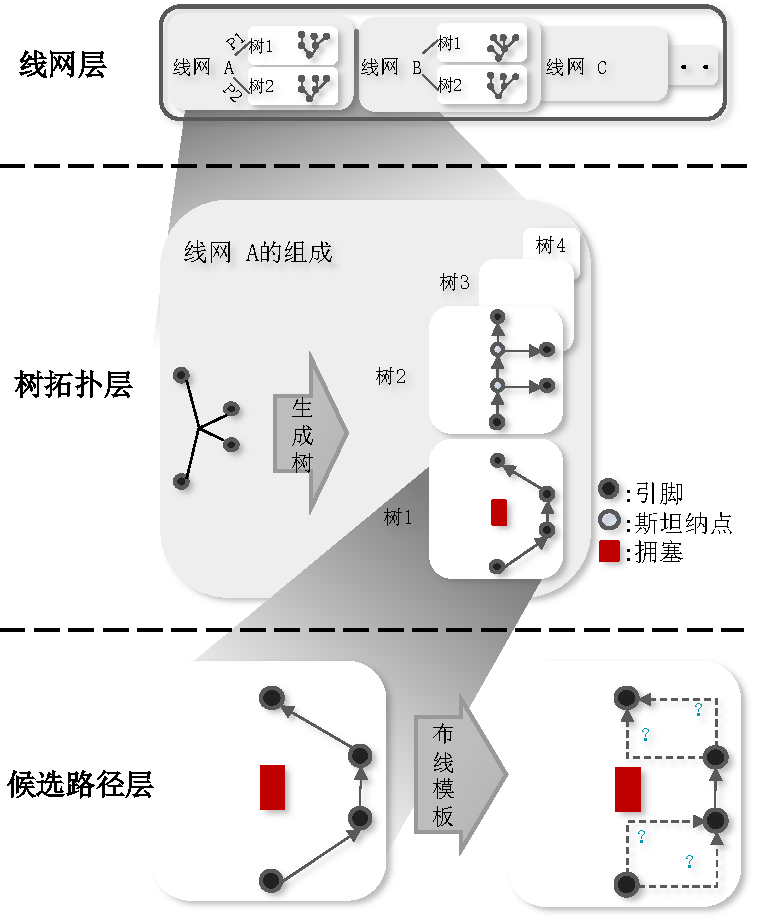
\includegraphics[width=0.95\textwidth]{image/chap03/树森林层级结构示意图.pdf}
    \caption{树森林层级结构示意图}
    \label{fig:chap3-forest-structure-placeholder}
\end{figure}

\subsection{RSMT候选生成}

RSMT候选由FLUTE算法快速生成\cite{10.1109/TCAD.2007.907068}。该候选以线长友好为主要特征，能够在多数低拥塞区域提供较短互连路径，是整个候选空间的低代价基线。

需要强调的是，RSMT候选虽具线长优势，但无法前瞻性的感知拥塞的发生。若仅依赖RSMT作为唯一拓扑，算法易在早期不可预知的情况下产生局部的拥塞，导致后续拥塞修复负担上升。因此，本文算法不将RSMT视为唯一的树生成算法候选，而将其作为树拓扑层中的一个候选选项。

\subsection{拥塞感知绕线树候选生成}

为补足RSMT对拥塞敏感性不足的问题，本文引入拥塞感知绕线树候选。具体做法为：先执行试布线，然后基于基于当前资源图得到初始的粗粒度的拥塞分布；针对潜在拥塞区域，对通过FLUTE算法获得的直角斯坦纳最小树执行边移动等绕线算法，可获得另一个树拓扑。由于候选生成过程中优先引导路径避开高拥塞边，因此该树拓扑具有良好的拥塞感知特性。并且，获取拥塞分布的环节并不局限于单一的拥塞感知算法，其他的拥塞预测算法也可以被集成到该流程中，形成更丰富的候选树森林。对应构建流程如图\ref{fig:chap3-forest-build-placeholder}所示。

该策略本质上是在初始化阶段获得不同指标优化导向的候选：
\begin{enumerate}
    \item RSMT候选偏线长友好；
    \item 绕线树候选偏拥塞友好。
\end{enumerate}
二者并存使后续训练可在较短路径与较低拥塞风险之间进行全局权衡，而不是在单一候选上被动调参。两类拓扑在典型线网上的几何差异可由图\ref{fig:chap3-two-tree-example-placeholder}直观看到。
此外，本文所讨论的全局布线问题未对时序等相关指标进行算法建模，因此在树森林构建阶段未引入时序相关的候选生成算法。但此算法框架具有较好的扩展性，也集成其他指标导向的树生成算法\cite{10.5555/3199700.3199776,10.1145/3394885.3431566}构建更丰富的候选树森林，以适配更复杂的多目标优化需求。

\begin{figure}[!htbp]
    \centering
    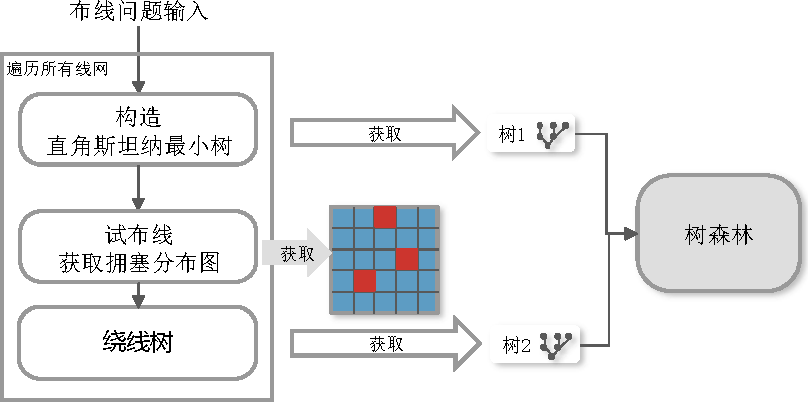
\includegraphics[width=0.95\textwidth]{image/chap03/候选树森林构建流程.pdf}
    \caption{候选树森林构建流程}
    \label{fig:chap3-forest-build-placeholder}
\end{figure}

\begin{figure}[!htbp]
    \centering
    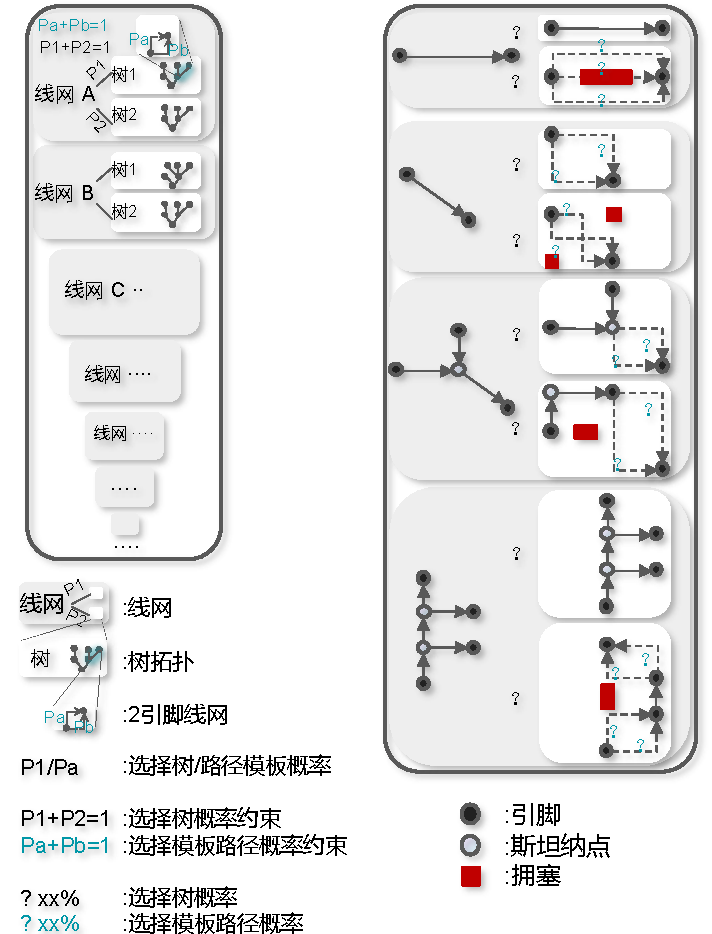
\includegraphics[width=0.70\textwidth]{image/chap03/双候选树拓扑对比示例.pdf}
    \caption{双候选树拓扑对比示例}
    \label{fig:chap3-two-tree-example-placeholder}
\end{figure}

\subsection{初始化阶段的算法流程}

设线网总数为 $|\mathcal{N}|$，每条线网平均引脚数为 $\bar{d}$。初始化阶段可分解为三步：
\begin{enumerate}
    \item 对每条线网调用FLUTE生成RSMT；
    \item 基于试探拥塞图执行拥塞感知候选生成；
    \item 按线网聚合形成树森林并完成候选索引映射。
\end{enumerate}

在工程实现中为降低索引开销，本文为每条线网维护连续内存布局的候选描述结构体，分别记录树拓扑边集、两引脚分解结果及路径模板索引范围。该设计为后续GPU侧批量张量化计算提供了基础。

\section{可微解析建模与优化目标}
\label{sec:chap3-diff-model}

\subsection{两层概率变量建模}

由前文候选树森林构建机制小节所述，树森林分为三个层次，后两个层次涉及候选选择问题。然而离散化的候选选择问题是非连续的，因此如果直接在离散域进行优化，将难以利用梯度信息，无法进行可微优化。本文采取DGR\cite{10.1145/3649329.3656530}的建模思路，将离散候选选择问题映射为可微优化问题，由此需要定义两层概率变量。

第一层为树拓扑选择概率。对每条线网 $n$，定义
\begin{equation}
    \mathbf{P}^{\mathrm{num}}_n=[P_{n1},P_{n2}],\quad
    P_{n1}+P_{n2}=1,\quad P_{nk}\in[0,1].
\end{equation}

第二层为两引脚模板路径选择概率。对线网 $n$ 中边 $e$ 的模板集合 $\mathcal{P}_{n,e}$，定义
\begin{equation}
    \mathbf{P}^{\mathrm{alpha}}_{n,e}=[P_{n,e}^{a},P_{n,e}^{b}],\quad
    P_{n,e}^{a}+P_{n,e}^{b}=1,\quad P_{n,e}^{a},P_{n,e}^{b}\in[0,1].
\end{equation}

通过上述连续变量，原始组合选择可转化为概率加权期望代价最小化问题。训练完成后再按高概率准则回到离散决策空间。

\subsection{联合代价函数构建}

本文目标函数由线长代价、通孔代价与拥塞溢出代价三部分组成：
\begin{equation}
    \mathcal{L}=\lambda_{wl}\mathcal{L}_{wl}+\lambda_{via}\mathcal{L}_{via}+\lambda_{of}\mathcal{L}_{of},
\end{equation}
其中 $\lambda_{wl}$、$\lambda_{via}$、$\lambda_{of}$ 为权重系数。

线长项可写为概率期望形式：
\begin{equation}
    \mathcal{L}_{wl}=\sum_{n\in\mathcal{N}}\sum_{k=1}^{2}P_{nk}\cdot WL(n,k,\mathbf{P}^{\mathrm{alpha}}),
\end{equation}
其中 $WL(n,k,\mathbf{P}^{\mathrm{alpha}})$ 表示在树 $k$ 与模板概率下的期望线长。

通孔项与之类似：
\begin{equation}
    \mathcal{L}_{via}=\sum_{n\in\mathcal{N}}\sum_{k=1}^{2}P_{nk}\cdot VIA(n,k,\mathbf{P}^{\mathrm{alpha}}).
\end{equation}

拥塞溢出项定义为全局边集合 $\mathcal{E}$ 上的超容量累积：
\begin{equation}
    \mathcal{L}_{of}=\sum_{g\in\mathcal{E}}\max\left(0,\;D_g(\mathbf{P}^{\mathrm{num}},\mathbf{P}^{\mathrm{alpha}})-C_g\right),
\end{equation}
其中 $D_g$ 为边 $g$ 的期望需求，$C_g$ 为边容量。

上述目标函数具备两方面优势：其一，可直接表达线长-通孔-拥塞多目标折中；其二，函数各项可通过并行归约计算，适合大规模线网场景下的GPU加速。

\subsection{概率回归与离散决策}

训练阶段采用梯度下降类优化器更新树拓扑概率与模板概率。在第 $r$ 轮迭代后，得到概率变量
\begin{equation}
    (\mathbf{P}^{\mathrm{num},(r+1)},\mathbf{P}^{\mathrm{alpha},(r+1)})
    =\operatorname{OptStep}\left((\mathbf{P}^{\mathrm{num},(r)},\mathbf{P}^{\mathrm{alpha},(r)}),\nabla\mathcal{L}^{(r)}\right).
\end{equation}

当满足以下任一条件时停止当前轮训练：
\begin{enumerate}
    \item 目标函数下降幅度小于阈值；
    \item 关键选择概率超过阈值（例如 $0.9$）；
    \item 达到设定最大迭代步数。
\end{enumerate}

停止训练后，对每组候选执行高概率离散化：
\begin{equation}
    t_n^*=\arg\max_{k\in\{1,2\}}P_{nk},
    \qquad
    p_{n,e}^*=\arg\max_{u\in\{a,b\}}P_{n,e}^{u}.
\end{equation}

\begin{figure}[!htbp]
    \centering
    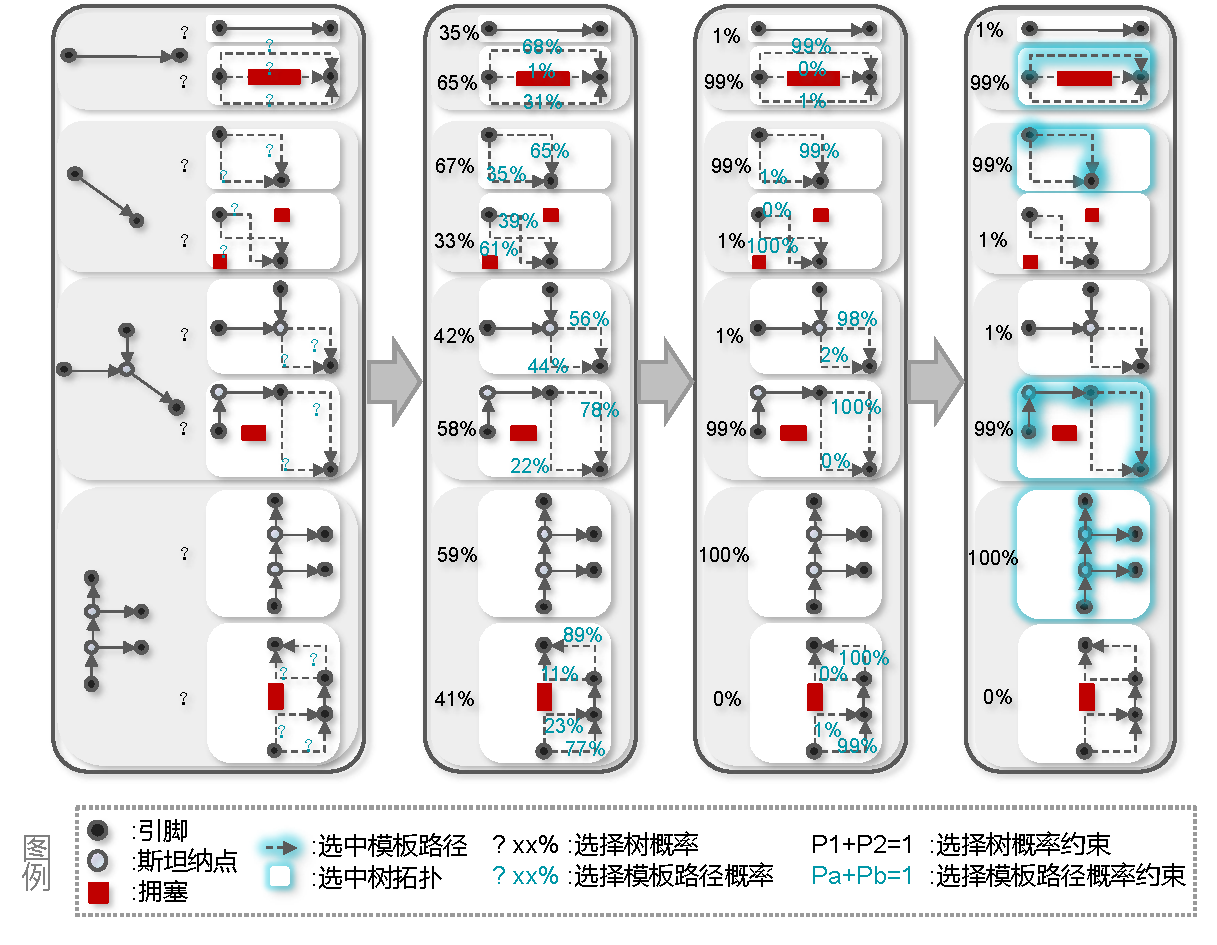
\includegraphics[width=0.95\textwidth]{image/chap03/树森林视角训练过程示意.pdf}
    \caption{树森林视角训练过程示意}
    \label{fig:chap3-training-forest-placeholder}
\end{figure}

\subsection{复杂度分析}

结合代码实现，复杂度分析需基于树森林扁平化与稀疏矩阵计算两部分展开。设线网数为 $N$，每个线网候选树数为 $K$（当前实现固定 $K=2$），每棵候选树平均两引脚边数为 $\bar{e}$，则全局两引脚边数近似为
\begin{equation}
    E \approx N\cdot K\cdot \bar{e}.
\end{equation}
在当前两层建模中，每条两引脚边对应 $M$ 个模板候选（当前实现固定 $M=2$），决策变量规模为 $E\cdot M$。构建需求矩阵时，\texttt{create\_masks\_fixed\_agian} 会遍历每个 $(e,m)$ 在网格上的经过位置并写入COO索引，若平均经过长度为 $\bar{\ell}$，则需求矩阵 $\mathbf{A}$ 的非零元数量满足
\begin{equation}
    \operatorname{nnz}(\mathbf{A})=\Theta(E\cdot M\cdot \bar{\ell}).
\end{equation}

单轮前向中，核心计算由三类矩阵操作组成：
\begin{enumerate}
    \item 树选择映射：$\mathbf{L}\mathbf{P}^{\mathrm{num}}_{\mathrm{flat}}$，复杂度约为 $O(\operatorname{nnz}(\mathbf{L}))=O(E)$；
    \item 需求聚合：$\mathbf{A}\mathbf{P}_{\mathrm{mix}}$，复杂度约为 $O(\operatorname{nnz}(\mathbf{A}))$；
    \item 通孔聚合：$\mathbf{v}\mathbf{P}_{\mathrm{mix}}$，复杂度约为 $O(E\cdot M)$。
\end{enumerate}
其中 $\mathbf{L}$ 为树到两引脚边映射矩阵，$\mathbf{P}_{\mathrm{mix}}$ 为展开后的联合概率向量。反向传播与前向同阶，因此每个epoch总体复杂度可写为
\begin{equation}
    O\big(\operatorname{nnz}(\mathbf{A}) + E\cdot M + G\big),
\end{equation}
其中 $G$ 为容量向量长度（当前实现为压缩后 $2XY$）。

进一步地，若记第 $r$ 轮参与优化线网比例为 $\eta^{(r)}=|\mathcal{N}^{(r)}|/|\mathcal{N}|$，则可近似写为
\begin{equation}
    O\Big(\eta^{(r)}\cdot\big(\operatorname{nnz}(\mathbf{A}) + E\cdot M + G\big)\Big).
\end{equation}
代码中每轮训练epoch上限为100，外层动态更新轮次上限设为5轮；因此当前版本总复杂度上界约为单次计算复杂度 $\times 500$。当后续扩展多轮动态更新时，$\eta^{(r)}$ 的下降趋势会直接决定总成本是否可控。

\subsection{数值稳定策略}

当前代码实现采用固定权重加Gumbel-Softmax退火策略，具体地，训练参数可记为logit矩阵
\begin{equation}
    \mathbf{Z}_{pattern}\in\mathbb{R}^{E\times 2},\qquad
    \mathbf{Z}_{tree}\in\mathbb{R}^{N\times 2},
\end{equation}
概率参数值在梯度下降优化的过程中有可能会出现负数，并且在负数出现的同时，一组候选内的其他概率参数可能随之出现大于1的情况。然而这违背了概率的定义，概率值必须在 $[0,1]$ 区间内，无论是负数的概率值还是大于1的概率值都不符合概率的定义。为了将非法概率值进行转换，需要对每组候选执行Softmax操作：
\begin{equation}
    P_{n,e}^{a}=\frac{\exp(Z_{n,e}^{a}/\tau)}{\exp(Z_{n,e}^{a}/\tau)+\exp(Z_{n,e}^{b}/\tau)},\qquad
    P_{n,e}^{b}=\frac{\exp(Z_{n,e}^{b}/\tau)}{\exp(Z_{n,e}^{a}/\tau)+\exp(Z_{n,e}^{b}/\tau)},
\end{equation}
由于Softmax操作引入了指数函数，因此经过指数转换后的每一项都介于区间 $[0,1]$ 之间。由此确保了概率参数值符合真实的概率定义。
此外，由于本研究的建模是将离散的布线选择问题转化为连续的概率优化问题，如果始终追求总的代价函数的最小化，则最终可能出现一组内的候选概率倾向于平均化的情况，这直接导致丧失了优化意义。因此在训练过程中需要逐步引导概率参数向离散化的决策空间收敛，即使得每组候选内的一个概率值趋近于1，另一个概率值趋近于0，由此可以在连续的问题建模中实现对离散决策问题的逼近。由此，需要在Softmax操作中引入温度参数 $\tau$，即Gumbel-Softmax操作：
\begin{equation}
    P_{n,e}^{a}=\frac{\exp(Z_{n,e}^{a}/\tau)}{\exp(Z_{n,e}^{a}/\tau)+\exp(Z_{n,e}^{b}/\tau)},\qquad
    P_{n,e}^{b}=\frac{\exp(Z_{n,e}^{b}/\tau)}{\exp(Z_{n,e}^{a}/\tau)+\exp(Z_{n,e}^{b}/\tau)}.
\end{equation}
通过调整温度参数 $\tau$ 的值，可以控制概率分布的平滑程度。当 $\tau$ 较大时，概率分布较为平滑，候选之间的概率值较为接近；当 $\tau$ 较小时，概率分布趋于尖锐，候选之间的概率值差异较大，更接近于离散化的决策空间。因此，在训练过程中逐步降低温度参数 $\tau$ 的值，可以引导概率参数向离散化的决策空间收敛，使得最终的优化结果更接近于实际的离散选择问题。当前代码实现中，初始温度参数设置为 $\tau^{(0)}=1.0$，并在每轮优化中逐渐降低温度参数：
\begin{equation}
    \tau^{(r+1)}=0.9\tau^{(r)}
\end{equation}
逐轮退火，实现前期探索、后期收敛的离散化逼近。

在最终的总损失设计上，代码中归一化的的联合优化目标表达式为：
\begin{equation}
    \mathcal{L}=500\cdot \sum\sigma(\mathbf{A}\mathbf{P}_{\mathrm{mix}}-\mathbf{c}) + 0.5\cdot\sum(\mathbf{A}\mathbf{P}_{\mathrm{mix}}) + 2\cdot\big(\mathbf{v}\mathbf{P}_{\mathrm{mix}}\big),
\end{equation}
其中第一项为溢出惩罚项、第二项为线长代价项、第三项为通孔代价项。


由于上述联合目标表达式，可以根据实际优化偏好设置不同的权重参数 $\lambda_{of},\lambda_{wl},\lambda_{via}$，以实现不同的优化导向（例如更强调拥塞修复或更强调线长优化）。当前版本中，本文采取CUGR2的权重参数设置，具体设置为 $\lambda_{of}=500$、$\lambda_{wl}=0.5$、$\lambda_{via}=2$，以确保在初始布线阶段根据最终的优化取向对不同的指标执行全局的权衡。


\section{拥塞感知的动态初始布线工作流构建}
\label{sec:chap3-dynamic}

前文已经给出了并行模板布线算法的可微建模与求解机制。本节进一步说明：本文未将该并行算法作为一次性求解步骤，为了发挥其全局优化优势，本文在工作流层面进行多轮复用。具体而言，每个轮次（round）都执行一次并行模板布线求解，随后依据该轮离散回写后的拥塞反馈，重构下一轮的树森林输入，由此形成拥塞感知的动态初始布线工作流。

需要注意区分单个并行求解过程内部的参数更新步以及树森林重构的区别。本文的树森林结构调整仅在一整轮模板布线结束后触发，而非在模板布线内部触发。围绕该轮次级闭环，本文采用两项协同策略：其一是针对拥塞线网执行动态候选树更新；其二是针对无拥塞线网执行动态规模缩减。

\subsection{树森林动态更新}

在第 $r$ 轮并行布线结束后，首先根据当前3D布线结果与资源容量，识别发生拥塞的线网集合：
\begin{equation}
    \mathcal{N}_{\mathrm{cong}}^{(r)}=\left\{n\in\mathcal{N}^{(r)}\mid\exists g\in\mathcal{P}_n^{(r)},\;D_g^{(r)}>C_g\right\},
\end{equation}
其中 $\mathcal{P}_n^{(r)}$ 为线网 $n$ 在第 $r$ 轮的路径集合，$D_g^{(r)}$ 为网格边 $g$ 的需求，$C_g$ 为容量。

对任意 $n\in\mathcal{N}_{\mathrm{cong}}^{(r)}$，本文不直接扩大候选规模，而是保持每个线网固定候选数，通过保留已选并替换未选的方式进行动态更新：
\begin{equation}
    \mathcal{T}_{n}^{(r+1)}=\left\{t_{n,\mathrm{sel}}^{(r)},\;\tilde{t}_{n,\mathrm{new}}^{(r+1)}\right\}.
\end{equation}
其中 $t_{n,\mathrm{sel}}^{(r)}$ 为第 $r$ 轮离散选择后的保留候选，$\tilde{t}_{n,\mathrm{new}}^{(r+1)}$ 为基于最新拥塞分布重新生成的拥塞感知候选树。该策略在不引入候选爆炸的前提下，为下一轮优化引入更贴合实时拥塞状态的拓扑，从而提升拥塞缓解能力。

\begin{figure}[!htbp]
    \centering
    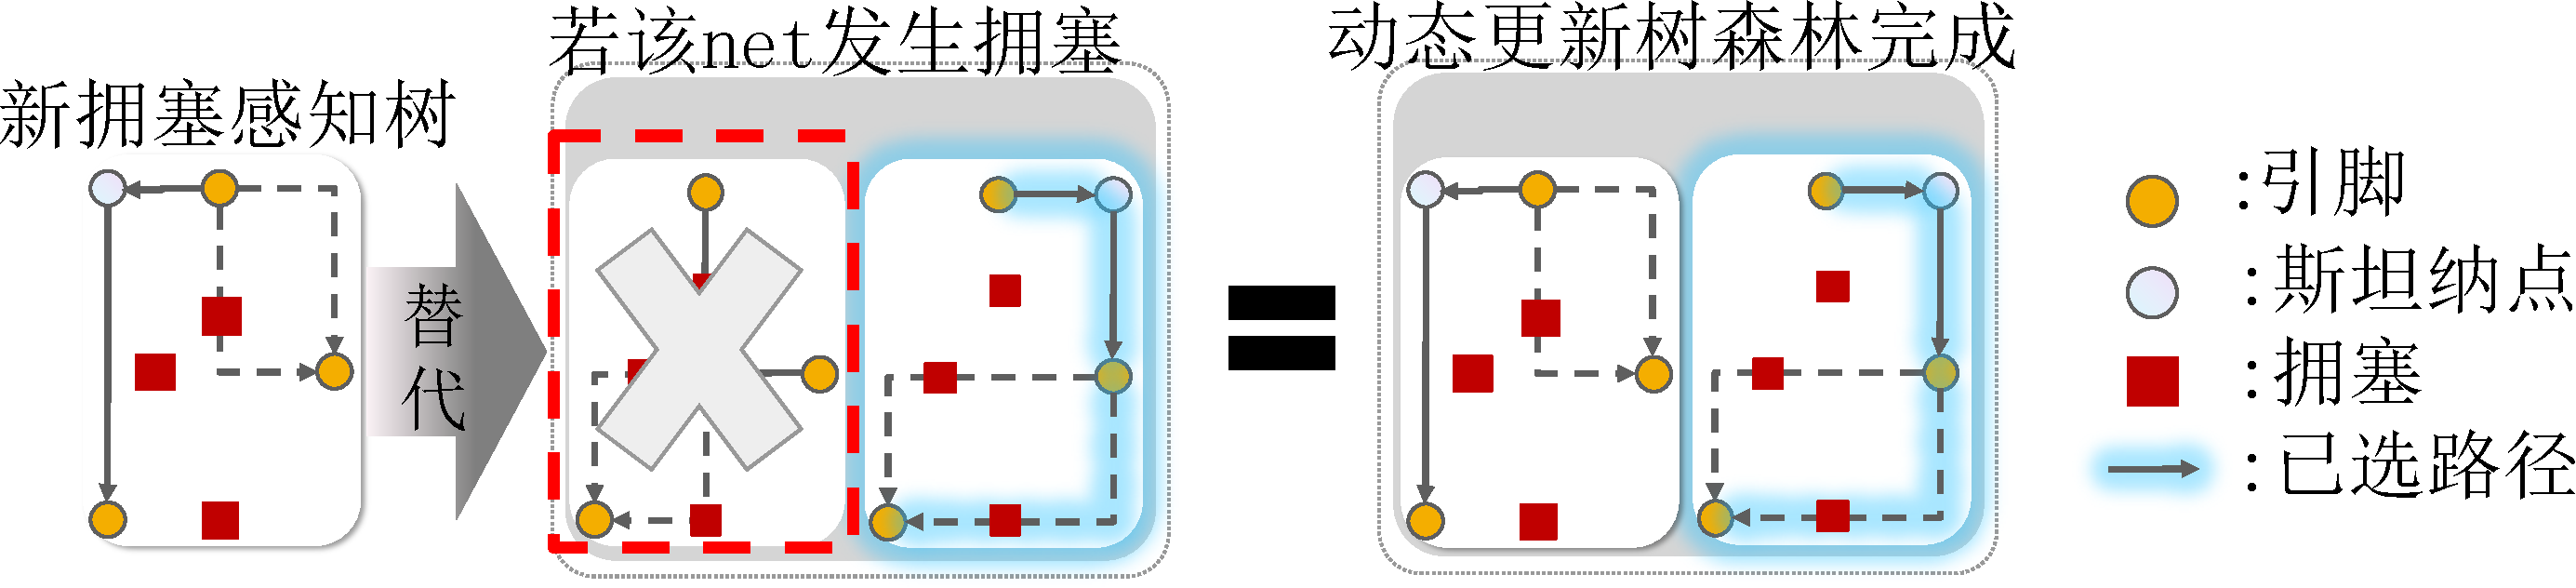
\includegraphics[width=0.95\textwidth]{image/chap03/动态更新树森林示例.pdf}
    \caption{拥塞线网的动态候选树更新示例}
    \label{fig:chap3-dynamic-update-example}
\end{figure}

如图\ref{fig:chap3-dynamic-update-example}所示，拥塞线网在新一轮的并行模板布线中不会重复使用原候选，而是注入新的拥塞感知候选树；该候选与上一轮保留候选共同构成下一轮树森林输入，使轮次间的搜索空间可持续向低拥塞方向迁移。

\subsection{树森林规模动态缩减}

与拥塞线网不同，对于已经无拥塞的线网，继续参与后续round优化收益有限。故在进入第 $r+1$ 轮前，定义无拥塞集合
\begin{equation}
    \mathcal{N}_{\mathrm{clean}}^{(r)}=\mathcal{N}^{(r)}\setminus\mathcal{N}_{\mathrm{cong}}^{(r)},
\end{equation}
并仅保留拥塞线网进入下一轮：
\begin{equation}
    \mathcal{N}^{(r+1)}=\mathcal{N}_{\mathrm{cong}}^{(r)}.
\end{equation}

从矩阵实现角度看，上述操作等价于将无拥塞线网对应的树级概率矩阵行、树-两引脚子网映射矩阵列以及需求矩阵相关列同时剔除，即对动态树森林执行规模缩减。这样可以显著降低后续轮次的优化变量规模与稀疏矩阵非零元规模。

\begin{figure}[!htbp]
    \centering
    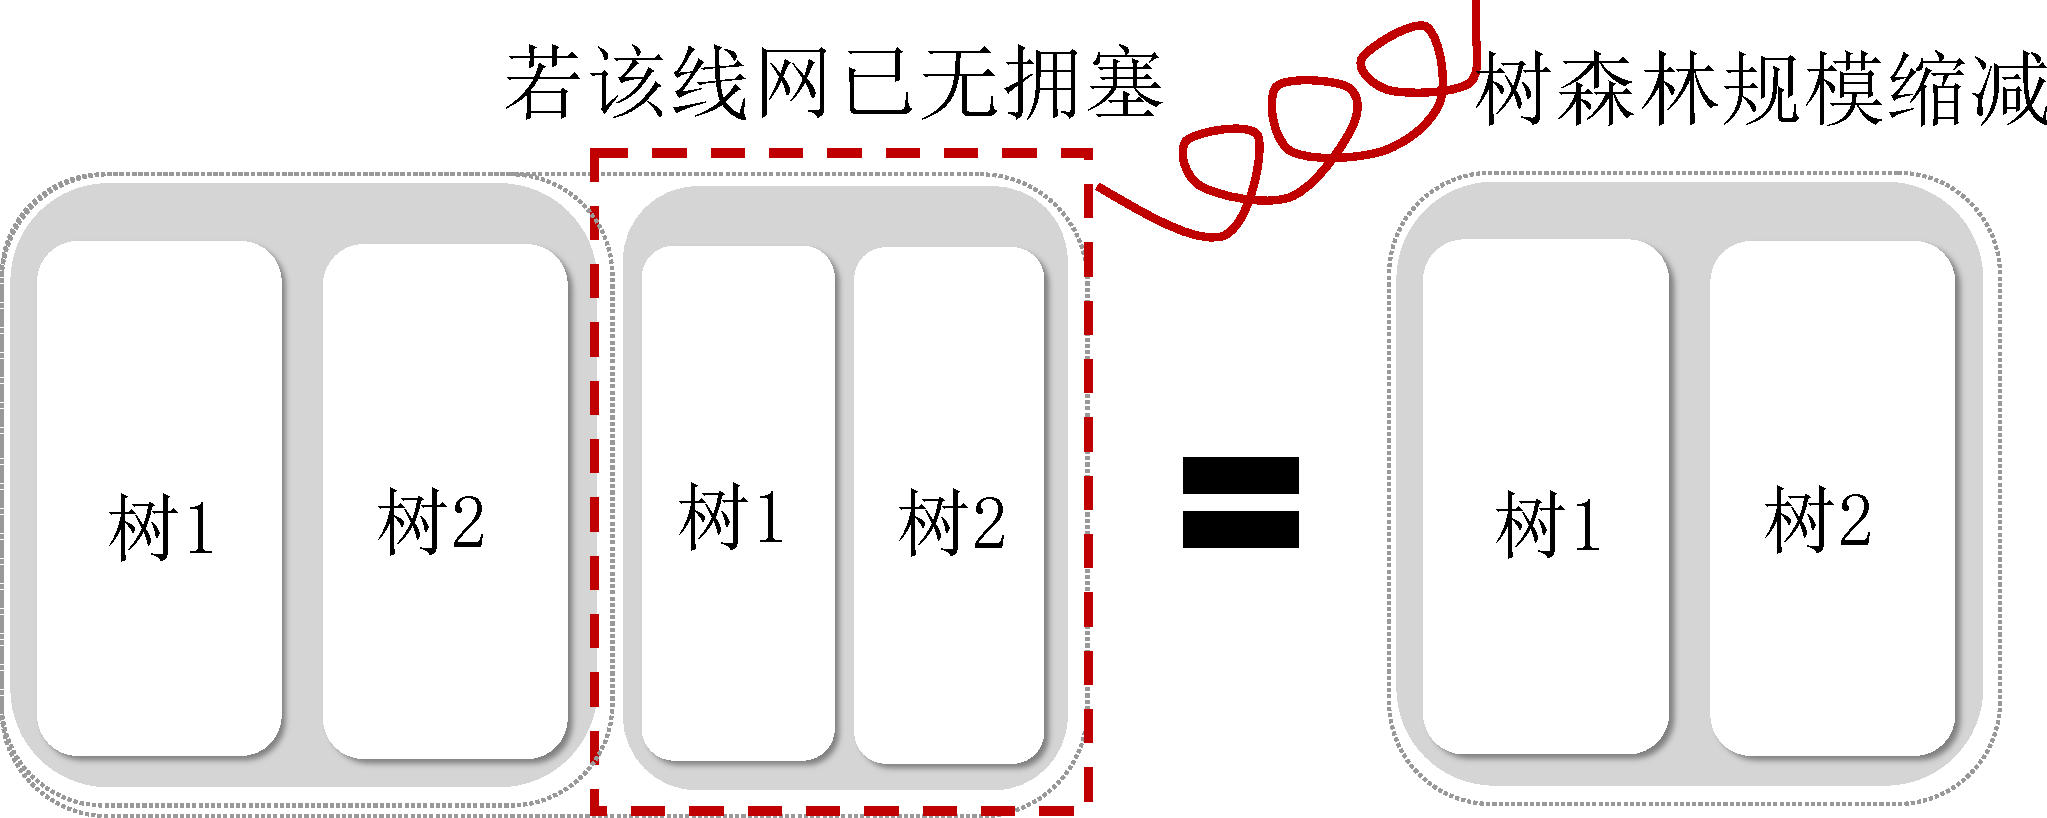
\includegraphics[width=0.70\textwidth]{image/chap03/动态缩减树森林规模示例.pdf}
    \caption{无拥塞线网的动态树森林规模缩减示例}
    \label{fig:chap3-dynamic-prune-example}
\end{figure}

定义第 $r$ 轮有效线网比例为
\begin{equation}
    \eta^{(r)}=\frac{|\mathcal{N}^{(r)}|}{|\mathcal{N}^{(0)}|},
\end{equation}
则第 $r$ 轮耗时可直观近似为
\begin{equation}
    T^{(r)}\approx \eta^{(r)}\,T^{(0)}.
\end{equation}
由于在大部分的设计中，通常仅有少部分线网持续拥塞，因此$\eta^{(r)}$ 会随round推进而迅速下降，总耗时不会随着round数量线性增长，而只呈现小幅增长。这也是多轮动态策略在保证布线质量提升的同时仍具可用工程效率的关键。

综合上述两项策略，动态工作流可归纳为如下跨轮次闭环：每轮先执行并行模板布线求解，再依据拥塞评估结果将线网划分为拥塞集合与无拥塞集合；对前者注入新的拥塞感知候选树以增强下一轮拥塞缓解能力，对后者执行行列缩减以降低后续计算规模。两项策略同时作用后，工作流在保持拥塞感知能力持续增强的同时，有效抑制了多轮优化带来的时间膨胀。

图\ref{fig:chap3-multi-round-training-placeholder}展示了树森林视角下的多轮次动态训练过程，即为图\ref{fig:chap3-training-forest-placeholder}基础上引入多轮次的树森林变化机制，在耗时增长有限代价下实现更强的拥塞缓解能力，从而提升最终布线质量。

\begin{figure}[!htbp]
    \centering
    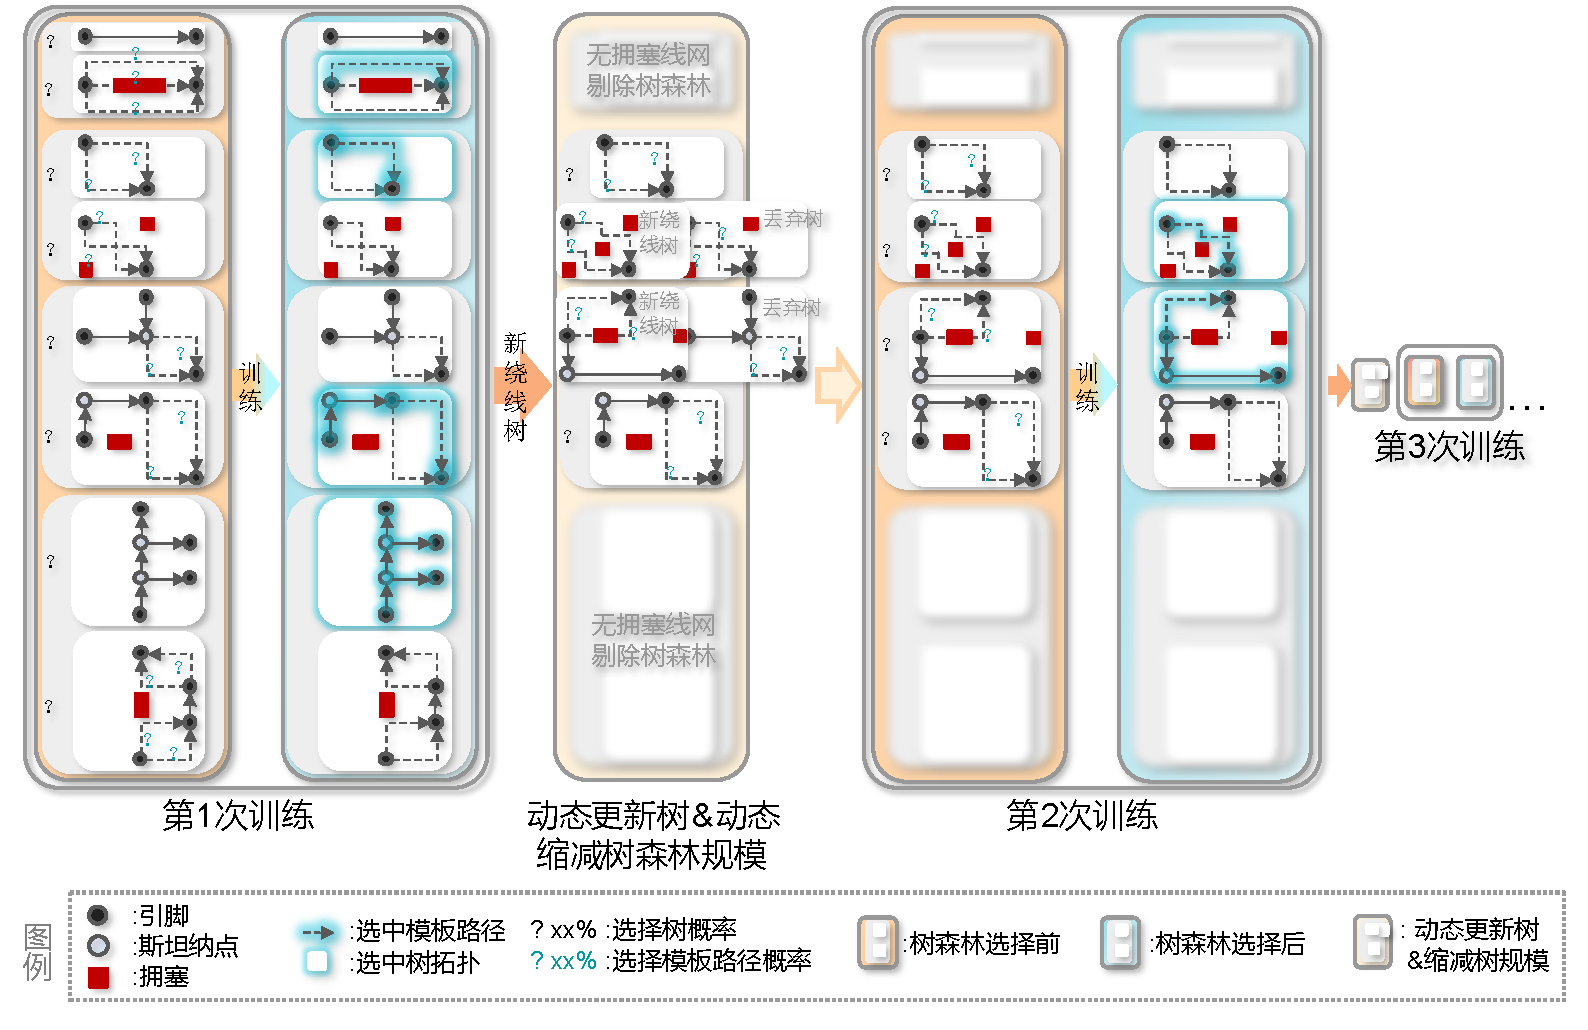
\includegraphics[width=0.95\textwidth]{image/chap03/树森林视角的多轮次动态训练过程示意.pdf}
    \caption{树森林视角的多轮次动态训练过程示意}
    \label{fig:chap3-multi-round-training-placeholder}
\end{figure}

\section{工程实现细节}
\label{sec:chap3-engineering}

\subsection{拥塞感知树生成}

从代码执行路径看，工程流程可划分为初始化树森林、拥塞驱动更新、矩阵化优化、离散回写四步。首先，对每个线网构建两棵候选树：一棵来自RSMT，另一棵来自随机化或拥塞驱动扰动；随后提取每棵树中的两引脚边，形成树森林基础数据。该步骤对应图\ref{fig:chap3-overall-flow-placeholder}与图\ref{fig:chap3-forest-build-placeholder}。

在拥塞感知树生成环节，核心不是直接替换全部候选，而是先通过试布线得到拥塞视图，再仅对拥塞线网执行候选更新。边移动（Edge Shifting）机制在此阶段通过局部绕行改变树边穿越位置，其作用是生成更拥塞友好的候选树，而不是独立的后处理步骤。图\ref{fig:chap3-edge-shift-placeholder}给出了该局部操作的几何示意，图\ref{fig:chap3-two-tree-example-placeholder}展示了线长友好候选与拥塞友好候选的对比结果。

\begin{figure}[!htbp]
    \centering
    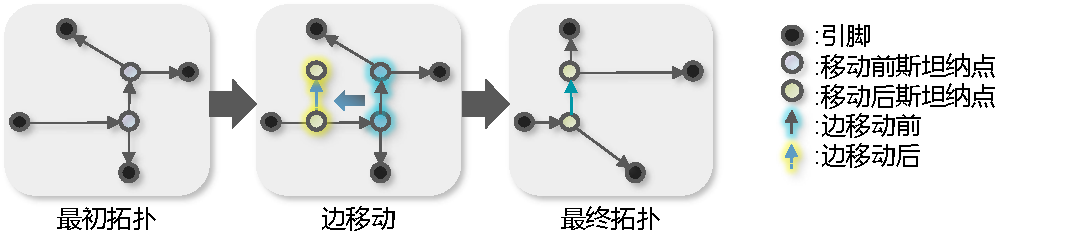
\includegraphics[width=0.95\textwidth]{image/chap03/边移动局部调整示意.pdf}
    \caption{边移动局部调整示意}
    \label{fig:chap3-edge-shift-placeholder}
\end{figure}

\subsection{树森林扁平化与映射矩阵构造}

在工程实现中，候选解首先以线网-候选树-两引脚子网三级集合进行组织，随后统一扁平化为全局两引脚子网索引集合，扁平化是为了建立统一的线网数据结构。设全局两引脚子网总数为 $E$，候选树总数为 $T$，构造树到两引脚子网的稀疏映射矩阵 $\mathbf{B}$：
\begin{equation}
    \mathbf{B}\in\{0,1\}^{E\times T},\qquad
    B_{e,t}=1\Leftrightarrow \text{两引脚子网 }e\text{ 属于候选树 }t.
\end{equation}

该映射矩阵用于将树级选择概率传播到两引脚子网级别。记树级概率向量为 $\mathbf{p}^{tree}\in\mathbb{R}^{T}$，则两引脚子网级继承概率可写为
\begin{equation}
    \hat{\mathbf{p}}=\mathbf{B}\mathbf{p}^{tree}.
\end{equation}
进一步，将 $\hat{\mathbf{p}}$ 在模板维度复制并与模板概率向量 $\mathbf{p}^{pat}\in\mathbb{R}^{EM}$ 逐元素相乘，可得到最终混合决策向量
\begin{equation}
    \mathbf{P}_{\mathrm{mix}}=\operatorname{repeat}(\hat{\mathbf{p}},M)\odot \mathbf{p}^{pat},
\end{equation}
其中 $M$ 为每条两引脚子网的候选模板数。图\ref{fig:chap3-forest-structure-placeholder}中的层次关系在工程上正是通过该扁平化与概率传播过程落地。

\subsection{稀疏映射矩阵与代价计算构造}

工程实现中，为了能够在优化阶段利用稀疏矩阵进行高效计算，需要构造需求稀疏映射矩阵与通孔映射矩阵。其基本思想是：遍历每个边-模板组合，枚举该组合经过的网格位置，并将经过需求写入COO格式索引。定义空间维度为 $(L,X,Y)$，则需求矩阵为
\begin{equation}
    \mathbf{A}\in\mathbb{R}^{(LXY)\times(EM)}.
\end{equation}

通过多维索引压平函数可得到行索引与列索引：
\begin{equation}
    r=((l\cdot X)+x)\cdot Y+y,\qquad c=e\cdot M+m.
\end{equation}
其中 $m$ 为模板编号（当前实现中 $m\in\{1,2\}$）。
据此构造 COO 稀疏张量后，前向计算中的需求项与通孔项分别写为
\begin{equation}
    \mathbf{d}=\mathbf{A}\mathbf{P}_{\mathrm{mix}},\qquad
    C_{via}=\mathbf{v}\mathbf{P}_{\mathrm{mix}}.
\end{equation}

\begin{figure}[!htbp]
    \centering
    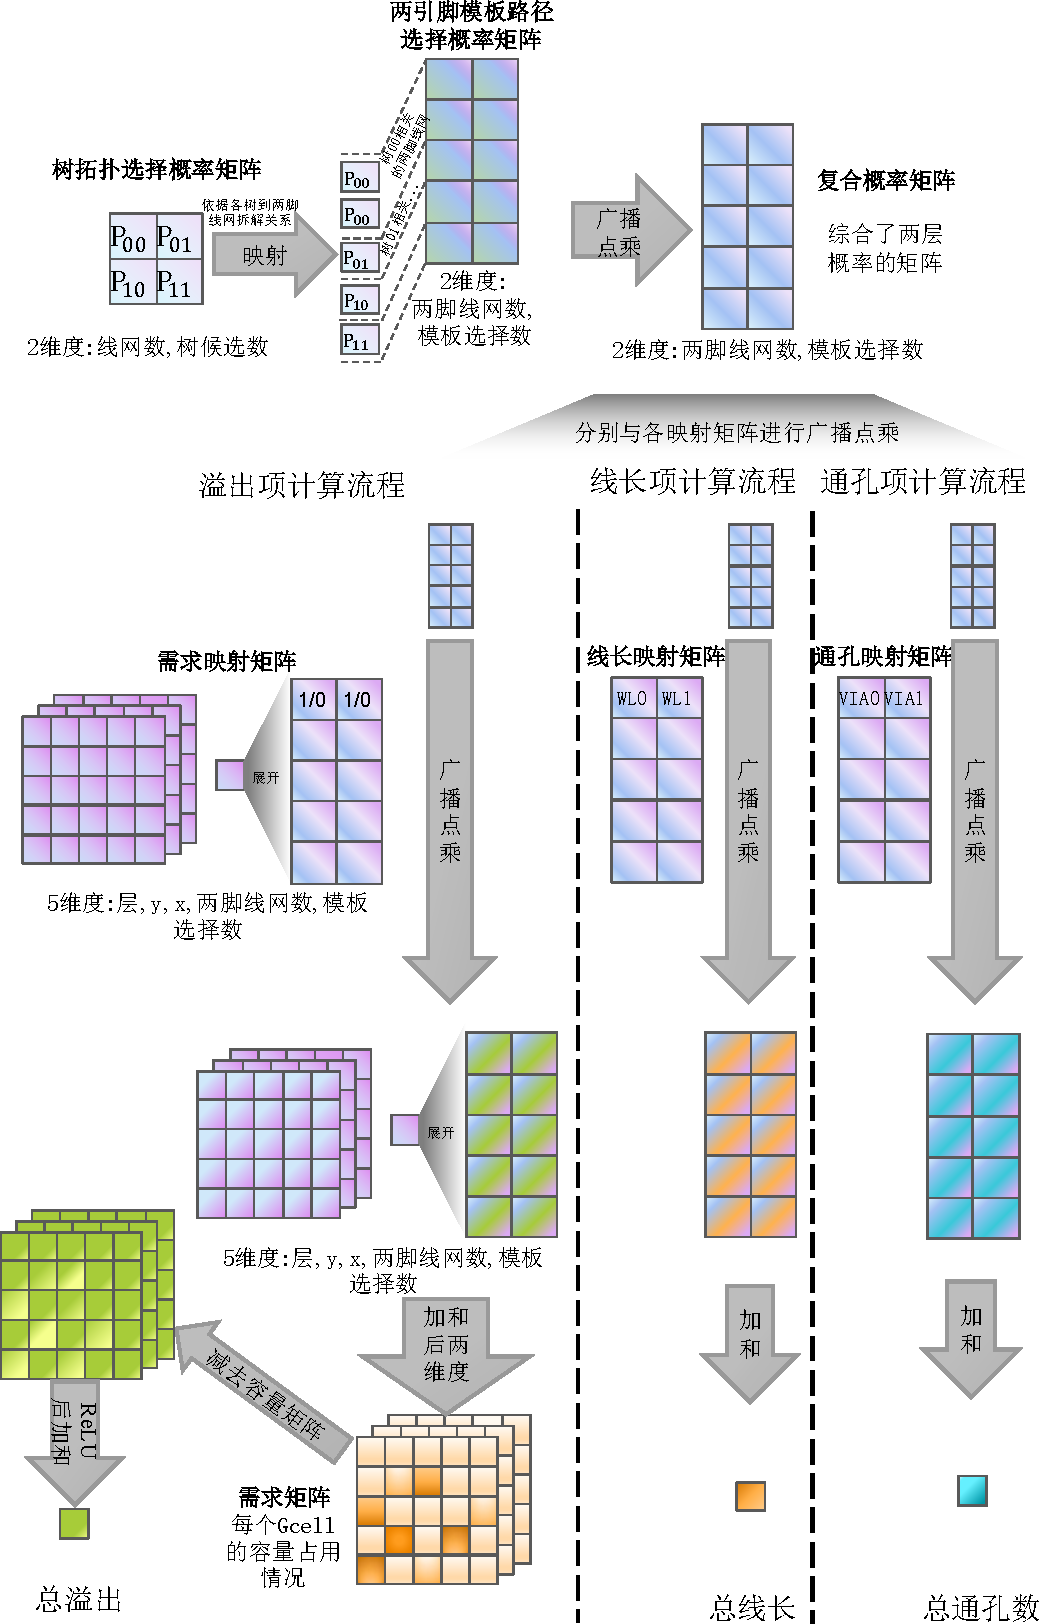
\includegraphics[width=0.98\textwidth]{image/chap03/并行化矩阵运算过程.pdf}
    \caption{并行化矩阵运算过程}
    \label{fig:chap3-matrix-op-flow}
\end{figure}

如图\ref{fig:chap3-matrix-op-flow}所示，矩阵化计算可进一步分解为三类代价通道：
\begin{enumerate}
    \item \textbf{Overflow cost（溢出代价）}：设容量向量为 $\mathbf{c}$，网格总数记为 $G=LXY$，则溢出代价采用可微惩罚函数
    \begin{equation}
        C_{of}=\sum_{g=1}^{G}\sigma\big(d_g-c_g\big),
    \end{equation}
    其中 $\sigma(\cdot)$ 为ReLU函数。该激活函数在需求逼近容量时也可产生连续梯度信号，有利于训练早期快速识别潜在拥塞区域。

    \item \textbf{Wirelength cost（线长代价）}：在当前矩阵实现中，线长项采用总需求代理，写为
    \begin{equation}
        C_{wl}=\sum_{g=1}^{G} d_g=\mathbf{1}^{\mathsf{T}}\mathbf{A}\mathbf{P}_{\mathrm{mix}}.
    \end{equation}
    该表达等价于对所有候选路径在网格上的占用进行全局累计，可作为线长优化的连续化近似。

    \item \textbf{Via cost（通孔代价）}：将每个候选路径对应的通孔开销组织为向量 $\mathbf{v}$，则
    \begin{equation}
        C_{via}=\mathbf{v}\mathbf{P}_{\mathrm{mix}}.
    \end{equation}
    该项显式约束层间切换次数，避免通过过多通孔换取局部拥塞缓解而导致后续制造代价上升。
\end{enumerate}

因此，联合目标可统一写为
\begin{equation}
    \mathcal{L}=\lambda_{of}C_{of}+\lambda_{wl}C_{wl}+\lambda_{via}C_{via}.
\end{equation}
这一形式将拥塞、线长与通孔三者纳入同一矩阵计算图中，实现了从概率决策到物理代价的并行映射。

\subsection{流程概述}

结合动态拥塞感知初始布线流程，整体可概括为如下步骤：
\begin{enumerate}
    \item 构建所有线网的初始双树候选，执行一次初始路由并提交到网格；
    \item 提取当前溢出线网集合，生成拥塞视图；
    \item 对溢出线网执行撤销提交、拥塞引导扰动与候选树重建，完成局部候选更新；
    \item 将更新后的候选森林扁平化，构造树-两引脚子网映射矩阵以及需求/通孔稀疏标记；
    \item 在连续概率空间中迭代优化树级与模板级参数，并通过退火策略逐步增强离散性；
    \item 依据最大概率准则完成离散化选择，得到树与模板的确定性决策；
    \item 依据离散结果重建每个线网的固定路由结构并重新提交路由树；
    \item 统计溢出并结束当前轮，进入下一轮动态更新（详见第\ref{sec:chap3-dynamic}节）。
\end{enumerate}

% 从实现正确性看，该流程依赖三类关键不变量：
% \begin{enumerate}
%     \item 索引一致性：通过 \texttt{assert(location\_count == location\_length)} 保证COO索引完整；
%     \item 拓扑一致性：每个两引脚边在固定模式回写时严格按先序遍历顺序消费，保证模式索引与边索引一一对应；
%     \item 资源一致性：溢出评估始终由需求-容量差值统一定义，轮次级动态过程如图\ref{fig:chap3-multi-round-training-placeholder}所示，仅缩减参与训练集合，不改变已提交解的连通性。
% \end{enumerate}

\section{并行全局布线层次分析}
\label{sec:chap3-parallel}

% \subsection{并行层级定义修正}

% 结合本工作代码实现，本文采用的两层并行应定义为：
% \begin{enumerate}
%     \item 数据级并行：在同一线网内部，并行评估该线网所有候选树与候选路径模式；
%     \item 线网级并行：将全部线网同时建模到同一个全局损失函数中，统一前向、统一反向、统一更新。
% \end{enumerate}
% 因此，线网级并行并非把线网分批异步调度再做局部决策，而是在一个联合目标中同步处理所有线网布线问题。

\subsection{数据级并行：基于GPU执行加速计算}

数据级并行指的是对每条两引脚边，两个L型模板的代价在张量中同时计算；对每个线网，候选树与边级模板概率通过矩阵乘法并行传播。具体包括：
\begin{enumerate}
    \item Gumbel-Softmax 并行生成边级模板概率与树级概率；
    \item 稀疏映射矩阵并行完成树概率 $\rightarrow$ 边概率传播；
    \item 需求矩阵并行完成边概率 $\rightarrow$ 网格需求聚合；
    \item 在GPU上并行完成损失计算与梯度反传。
\end{enumerate}

这一层并行化本质是利用GPU对矩阵运算实现并行加速，避免串行计算的低效，从而对模板布线过程进行有效加速。

\subsection{线网级并行：全局视角衡量候选优劣}

线网级并行对应问题建模层。所有线网共享同一组全局容量约束，并在同一个损失函数中共同优化：
\begin{equation}
    \mathcal{L}_{global}=\sum_{g}\phi\big(D_g(\mathbf{P}_{\mathrm{mix}})-C_g\big)+\sum_g D_g(\mathbf{P}_{\mathrm{mix}})+\psi(\mathbf{P}_{\mathrm{mix}}).
\end{equation}
其中 $D_g(\mathbf{P}_{\mathrm{mix}})$ 由所有线网共同贡献。由于该目标函数不可分解为彼此独立的单线网子问题，模型天然地在一次前向中同时考虑所有线网对全局拥塞的耦合影响。这正是本文线网级并行的核心含义。

% \subsection{并行效率与实现边界}

% 在当前实现中，并行效率主要受三类因素影响：
% \begin{enumerate}
%     \item 稀疏矩阵非零元规模（决定矩阵乘法开销）；
%     \item 网格规模与容量向量长度（决定全局归约开销）；
%     \item 概率退火速度（影响训练后期梯度稳定性与收敛速度）。
% \end{enumerate}

通过以上两层次的并行化设计，当前方案通过数据级并行确保利用GPU的并行计算吞吐能力、线网级并行保证全局视角选择更为合适的树拓扑以实现耦合优化，实现了效率与质量的统一。

\section{实验设置与结果分析}
\label{sec:chap3-exp}

\subsection{实验目标与评价维度}

本节实验围绕两个问题展开：
\begin{enumerate}
    \item 所提动态拥塞感知初始布线流程是否能有效降低拥塞线网数量与溢出；
    \item 在引入动态更新与动态缩减后，算法能否在可接受开销内取得稳定收益。
\end{enumerate}

评价指标采用全局布线常用指标：总线长（Wirelength）、通孔数（Via）、总溢出（Overflow）与运行时间（Runtime）。其中，溢出指标作为本章核心评价维度，用于衡量流程对拥塞风险的抑制能力。

\subsection{实验平台与测试基准}

实验基准覆盖ISPD'18、ISPD'19、ICCAD'19 Metal5受限版本与ISPD'24四类公开测试集，能够覆盖不同规模与拥塞复杂度场景。表\ref{tab:chap3-benchmark-placeholder}给出了统一字段下的规模统计：ISPD'18与ISPD'19提供通用公开算例，ICCAD'19 Metal5受限版本提供层数受限算例，ISPD'24提供工业规模算例。对比对象选择代表性解析式与组合式全局布线方法，包括DGR\cite{10.1145/3649329.3656530}与CUGR2\cite{10.1109/DAC56929.2023.10247702}，其中DGR为基于CUGR2的使用libtorch的复现版本。平台配置采用高性能CPU与GPU异构环境，以保证可微求解流程的并行执行效率。

\begin{table}[!htbp]
    \centering
    \caption{实验平台配置}
    \label{tab:chap3-platform-placeholder}
    \begin{tabular}{p{0.18\textwidth}p{0.26\textwidth}p{0.48\textwidth}}
        \hline
        类别 & 配置项 & 具体配置 \\
        \hline
        硬件 & CPU & 2 $\times$ Intel Xeon Gold 6530，64 物理核 / 128 逻辑核，主频范围 0.8--4.0 GHz \\
        硬件 & 内存 & 1.0 TiB \\
        硬件 & GPU & NVIDIA RTX 4090 \\
        系统 & 操作系统 & Debian GNU/Linux forky/sid \\
        系统 & 内核版本 & Linux 5.4.0-42-generic \\
        软件栈 & Python & Python 3.13.12 \\
        \hline
    \end{tabular}
\end{table}

\begin{table}[!htbp]
    \centering
    \caption{测试基准与规模统计}
    \label{tab:chap3-benchmark-placeholder}
    \small
    \setlength{\tabcolsep}{4.2pt}
    \renewcommand{\arraystretch}{1.10}
    \begin{tabular}{l c c r r r}
        \hline
        测试用例 & 网格规模 ($X\times Y$) & 层数 & 线网数 & 单元数 & 端口数 \\
        \hline
        \texttt{ispd18\_test1} & $65\times67$ & 9 & 3153 & 8879 & 0 \\
        \texttt{ispd18\_test2} & $216\times201$ & 9 & 36834 & 35913 & 1211 \\
        \texttt{ispd18\_test3} & $329\times247$ & 9 & 36700 & 35977 & 1211 \\
        \texttt{ispd18\_test4} & $592\times403$ & 9 & 72410 & 72094 & 1211 \\
        \texttt{ispd18\_test5} & $619\times613$ & 9 & 72394 & 71954 & 1211 \\
        \texttt{ispd18\_test6} & $571\times354$ & 9 & 107701 & 107919 & 1211 \\
        \texttt{ispd18\_test7} & $905\times883$ & 9 & 179863 & 179881 & 1211 \\
        \texttt{ispd18\_test8} & $905\times883$ & 9 & 179863 & 192003 & 1211 \\
        \texttt{ispd18\_test9} & $606\times522$ & 9 & 178858 & 192911 & 1211 \\
        \texttt{ispd18\_test10} & $606\times522$ & 9 & 182000 & 290386 & 1211 \\
        \texttt{ispd19\_test1} & $98\times97$ & 9 & 3153 & 8879 & 0 \\
        \texttt{ispd19\_test2} & $581\times392$ & 9 & 72410 & 72094 & 1211 \\
        \texttt{ispd19\_test3} & $130\times130$ & 9 & 8953 & 8283 & 57 \\
        \texttt{ispd19\_test4} & $534\times517$ & 5 & 151612 & 146442 & 4802 \\
        \texttt{ispd19\_test5} & $302\times302$ & 5 & 29416 & 28920 & 360 \\
        \texttt{ispd19\_test6} & $905\times883$ & 9 & 179863 & 179881 & 1211 \\
        \texttt{ispd19\_test7} & $1053\times1011$ & 9 & 358720 & 359746 & 2216 \\
        \texttt{ispd19\_test8} & $1202\times1138$ & 9 & 537577 & 539611 & 3221 \\
        \texttt{ispd19\_test9} & $1337\times1433$ & 9 & 895252 & 899341 & 3221 \\
        \texttt{ispd19\_test10} & $1337\times1433$ & 9 & 895253 & 899404 & 3221 \\
        \texttt{ispd18\_test5\_metal5} & $619\times613$ & 5 & 72394 & 71954 & 1211 \\
        \texttt{ispd18\_test8\_metal5} & $905\times883$ & 5 & 179863 & 192003 & 1211 \\
        \texttt{ispd18\_test10\_metal5} & $606\times522$ & 5 & 182000 & 290386 & 1211 \\
        \texttt{ispd19\_test7\_metal5} & $1053\times1011$ & 5 & 358720 & 359746 & 2216 \\
        \texttt{ispd19\_test8\_metal5} & $1202\times1138$ & 5 & 537577 & 539611 & 3221 \\
        \texttt{ispd19\_test9\_metal5} & $1337\times1433$ & 5 & 895252 & 899341 & 3221 \\
        \texttt{ariane133\_51} & $844\times1144$ & 10 & 128673 & 121794 & 435 \\
        \texttt{ariane133\_68} & $716\times971$ & 10 & 127026 & 120202 & 435 \\
        \texttt{bsg\_chip} & $1532\times2077$ & 10 & 768239 & 714938 & 42 \\
        \texttt{mempool\_tile} & $475\times644$ & 10 & 135919 & 128515 & 1148 \\
        \texttt{nvdla} & $1240\times1682$ & 10 & 176765 & 166393 & 684 \\
        \hline
    \end{tabular}
\end{table}

\subsection{主实验结果}

本文动态拥塞感知初始布线流程在测试集上，相对代表性解析式与组合式方法表现出更强拥塞抑制能力。表\ref{tab:chap3-main-result}展示了我们的方案与 CUGR2 和 DGR 在模板布线上的指标对比。按表\ref{tab:chap3-main-result}中31个测试用例的溢出数据统计，本文方法相较DGR的溢出降低约24.9\%，相较CUGR2的溢出降低约44.1\%。该结果表明，在初始布线阶段前置拥塞感知并引入动态闭环，有助于减少中后期高代价修复压力。

同时，从运行时间角度看，多轮动态流程会带来额外计算开销，但由于动态缩减机制逐轮减少训练线网规模，时间开销增长呈受控态势。实践中，该受控增长换取了显著拥塞收益，整体上体现出质量与效率的更优平衡。

\begin{table}[!htbp]
    \centering
    \caption{质量指标对比}
    \label{tab:chap3-main-result}
    \setlength{\tabcolsep}{4pt}
    \renewcommand{\arraystretch}{1.08}
    \resizebox{\textwidth}{!}{
        \begin{tabular}{l rrr rrr rrr}
            \toprule
            \multirow{2}{*}{测试用例} & \multicolumn{3}{c}{线长} & \multicolumn{3}{c}{通孔数} & \multicolumn{3}{c}{溢出} \\
            \cmidrule(lr){2-4} \cmidrule(lr){5-7} \cmidrule(lr){8-10}
                                    & CUGR2            & DGR               & 本文方法        & CUGR2            & DGR               & 本文方法        & CUGR2          & DGR             & 本文方法      \\
            \midrule
            ispd18\_test1          & \textbf{409081}   & \textbf{409081}   & \textbf{409081}  & \textbf{32454}   & \textbf{32454}    & \textbf{32454}   & \textbf{0}      & \textbf{0}      & \textbf{0}    \\
            ispd18\_test2          & \textbf{7603188}  & \textbf{7603188}  & \textbf{7603188} & \textbf{357967}  & \textbf{357967}   & \textbf{357967}  & \textbf{0}      & \textbf{0}      & \textbf{0}    \\
            ispd18\_test3          & \textbf{8531627}  & \textbf{8531627}  & \textbf{8531627} & 360466          & \textbf{360454}   & \textbf{360454}  & \textbf{0}      & \textbf{0}      & \textbf{0}    \\
            ispd18\_test4          & \textbf{25620922} & 25635707          & 25635647         & 772767          & 772777            & \textbf{772746}  & 1174           & \textbf{0}      & \textbf{0}    \\
            ispd18\_test5          & \textbf{26719280} & 26740190          & 26740460         & \textbf{896347}  & 896803            & 896795           & 75             & \textbf{0}      & \textbf{0}    \\
            ispd18\_test6          & \textbf{34220480} & 34241555          & 34253465         & 1347248         & 1347311           & \textbf{1347210} & 428            & 71              & \textbf{0}    \\
            ispd18\_test7          & \textbf{62761893} & 62817858          & 62824848         & \textbf{2206523} & 2207719           & 2207628          & 27862          & 8783            & \textbf{1058} \\
            ispd18\_test8          & \textbf{62964888} & 63029328          & 63042633         & \textbf{2251453} & 2252852           & 2252911          & 27876          & 8771            & \textbf{960}  \\
            ispd18\_test9          & \textbf{52494024} & 52502349          & 52499784         & \textbf{2241545} & 2242142           & 2242107          & 1011           & 31              & \textbf{0}    \\
            ispd18\_test10         & \textbf{65090544} & 65154399          & 65187579         & \textbf{2368014} & 2370408           & 2370994          & \textbf{1796}   & 5947            & 6069           \\
            ispd19\_test1          & \textbf{601511}   & \textbf{601511}   & \textbf{601511}  & \textbf{38499}   & \textbf{38499}    & \textbf{38499}   & \textbf{0}      & \textbf{0}      & \textbf{0}    \\
            ispd19\_test2          & \textbf{23943128} & 23955842          & 23959649         & \textbf{808496}  & 808731            & 808740           & 324            & 71              & \textbf{14}   \\
            ispd19\_test3          & \textbf{774750}   & 774930            & 774930           & \textbf{65079}   & 65103             & 65103            & 7              & \textbf{4}      & \textbf{4}    \\
            ispd19\_test4          & \textbf{25287922} & 25658050          & 25861815         & \textbf{755438}  & 761515            & 764535           & 214888         & 186082          & \textbf{147072} \\
            ispd19\_test5          & \textbf{4220085}  & 4254615           & 4257945          & \textbf{156680}  & 157145            & 157235           & 29060          & 21128           & \textbf{20585} \\
            ispd19\_test6          & \textbf{63649578} & 63702168          & 63728853         & \textbf{2045541} & 2047428           & 2047201          & 36860          & 8739            & \textbf{1210} \\
            ispd19\_test7          & \textbf{117043233} & 117206163         & 117242118        & \textbf{3808931} & 3818624           & 3818762          & \textbf{14401} & 33020           & 14747          \\
            ispd19\_test8          & \textbf{180606119} & 180803724         & 180787644        & \textbf{6298931} & 6299926           & 6300058          & 20059          & 145             & \textbf{0}    \\
            ispd19\_test9          & \textbf{272442799} & 272513104         & 272519239        & \textbf{10488012} & 10491391          & 10491625         & 361            & 206             & \textbf{0}    \\
            ispd19\_test10         & \textbf{268638004} & 268780621         & 268785745        & \textbf{9646345} & 9647443           & 9647812          & 23318          & 7318            & \textbf{6094} \\
            ispd18\_test5\_metal5 & \textbf{25555635} & 25703970          & 25709175         & \textbf{873683}  & 876918            & 876921           & 63993          & 43113           & \textbf{37995} \\
            ispd18\_test8\_metal5 & \textbf{58877869} & 59282854          & 59346019         & \textbf{2171062} & 2178494           & 2180373          & 116252         & 81451           & \textbf{53893} \\
            ispd18\_test10\_metal5 & \textbf{62480282} & 62833202          & 62983817         & \textbf{2260680} & 2268622           & 2271584          & \textbf{46630}  & 102268          & 101799         \\
            ispd19\_test7\_metal5 & \textbf{101591635} & 101996635         & 102138325        & \textbf{3787758} & 3803429           & 3807167          & 137601         & 124958          & \textbf{114034} \\
            ispd19\_test8\_metal5 & \textbf{166178884} & 166808599         & 166996084        & \textbf{6236992} & 6249606           & 6253175          & 353260         & 288230          & \textbf{252105} \\
            ispd19\_test9\_metal5 & \textbf{254881352} & 255467552         & 255691772        & \textbf{10396151} & 10413501          & 10417961         & 346328         & 290530          & \textbf{264645} \\
            ariane133\_51          & \textbf{18593148} & 18626426          & 18629236         & \textbf{1004753} & 1007282           & 1008121          & 5430           & 382             & \textbf{66}   \\
            ariane133\_68          & \textbf{18895608} & 18970596          & 18969990         & \textbf{956737}  & 960909            & 962133           & 22159          & 2427            & \textbf{754}  \\
            bsg\_chip              & \textbf{116192206} & 116649953         & 116782852        & \textbf{6319828} & 6337012           & 6341978          & 224133         & 119506          & \textbf{52542} \\
            mempool\_tile          & \textbf{16820490} & 16866961          & 16874116         & \textbf{1135001} & 1139491           & 1141860          & 5689           & 3074            & \textbf{1814} \\
            nvdla                  & \textbf{42556632} & 42917424          & 43086075         & \textbf{1452197} & 1458950           & 1461924          & 300135         & 167646          & \textbf{52154} \\
            \midrule
            平均 & \textbf{0.997168} & 0.999355          & 1.000000         & \textbf{0.998059} & 0.999604           & 1.000000          & 1.789204       & 1.331341        & \textbf{1.000000} \\
            \bottomrule
        \end{tabular}
    }
\end{table}

\subsection{与DGR的耗时对比}

为评估拥塞感知初始工作流的耗时代价，本文统计了DGR与初始布线工作流在31个测试用例上的运行时间，如表\ref{tab:chap3-runtime-vs-dgr}所示。表中模板布线耗时对应模板布线阶段的耗时，总耗时对应完整布线流程耗时。

\begin{table}[!htbp]
    \centering
    \caption{初始布线工作流与DGR耗时对比}
    \label{tab:chap3-runtime-vs-dgr}
    \small
    \setlength{\tabcolsep}{4.5pt}
    \renewcommand{\arraystretch}{1.06}
    \resizebox{\textwidth}{!}{
        \begin{tabular}{l r r r r}
            \toprule
            \multirow{2}{*}{测试用例} & \multicolumn{2}{c}{并行模板布线耗时/s} & \multicolumn{2}{c}{总耗时/s} \\
            \cmidrule(lr){2-3} \cmidrule(lr){4-5}
            & DGR & 本文方法 & DGR & 本文方法 \\
            \midrule
            \texttt{ispd18\_test1} & 0.406 & 0.385 & 0.771 & 0.583 \\
            \texttt{ispd18\_test2} & 2.449 & 1.974 & 4.438 & 3.520 \\
            \texttt{ispd18\_test3} & 3.960 & 2.988 & 6.628 & 4.699 \\
            \texttt{ispd18\_test4} & 8.102 & 9.085 & 14.505 & 13.951 \\
            \texttt{ispd18\_test5} & 9.970 & 7.287 & 16.479 & 12.495 \\
            \texttt{ispd18\_test6} & 11.481 & 11.316 & 19.968 & 17.291 \\
            \texttt{ispd18\_test7} & 20.980 & 22.589 & 39.438 & 36.520 \\
            \texttt{ispd18\_test8} & 21.452 & 23.536 & 42.418 & 37.731 \\
            \texttt{ispd18\_test9} & 18.547 & 17.061 & 33.700 & 28.286 \\
            \texttt{ispd18\_test10} & 24.852 & 38.808 & 48.740 & 56.058 \\
            \texttt{ispd19\_test1} & 0.594 & 0.416 & 0.867 & 0.622 \\
            \texttt{ispd19\_test2} & 8.566 & 9.327 & 15.794 & 14.394 \\
            \texttt{ispd19\_test3} & 1.347 & 2.718 & 1.985 & 3.110 \\
            \texttt{ispd19\_test4} & 12.242 & 27.684 & 28.157 & 38.278 \\
            \texttt{ispd19\_test5} & 2.883 & 4.884 & 4.760 & 6.198 \\
            \texttt{ispd19\_test6} & 23.178 & 24.068 & 40.585 & 38.347 \\
            \texttt{ispd19\_test7} & 48.208 & 53.710 & 85.605 & 79.901 \\
            \texttt{ispd19\_test8} & 45.531 & 47.037 & 87.059 & 79.077 \\
            \texttt{ispd19\_test9} & 72.277 & 70.102 & 138.643 & 122.374 \\
            \texttt{ispd19\_test10} & 87.520 & 69.749 & 169.474 & 127.147 \\
            \texttt{ispd18\_test5\_metal5} & 9.525 & 16.659 & 17.827 & 22.711 \\
            \texttt{ispd18\_test8\_metal5} & 26.336 & 44.830 & 50.760 & 62.391 \\
            \texttt{ispd18\_test10\_metal5} & 23.532 & 54.194 & 56.098 & 80.623 \\
            \texttt{ispd19\_test7\_metal5} & 39.872 & 53.806 & 87.752 & 91.396 \\
            \texttt{ispd19\_test8\_metal5} & 49.075 & 78.097 & 107.168 & 128.112 \\
            \texttt{ispd19\_test9\_metal5} & 71.800 & 105.283 & 156.127 & 177.494 \\
            \texttt{ariane133\_51} & 11.098 & 13.910 & 23.369 & 24.676 \\
            \texttt{ariane133\_68} & 13.737 & 14.236 & 26.481 & 23.929 \\
            \texttt{bsg\_chip} & 83.150 & 111.166 & 162.301 & 168.232 \\
            \texttt{mempool\_tile} & 12.295 & 14.165 & 23.919 & 22.416 \\
            \texttt{nvdla} & 36.782 & 43.522 & 72.248 & 64.782 \\
            \midrule
            平均比例 & 80.6\% & 100.0\% & 99.8\% & 100.0\% \\
            \bottomrule
        \end{tabular}
    }
\end{table}

从表\ref{tab:chap3-runtime-vs-dgr}可见，初始布线工作流在并行模板布线阶段的平均耗时约为DGR的1.24倍，这与本文执行5次并行模板布线而DGR仅执行1次并行模板布线一致。更重要的是，受益于动态缩减树森林规模与已收敛线网剔除策略，流程总耗时并未随迭代次数线性增长，平均总耗时仅为DGR的100.2\%，即仅增加约0.2\%。这说明动态缩减策略能够有效抑制多轮迭代带来的时间膨胀，在显著改善拥塞的同时保持较高运行效率。

% \subsection{消融实验：动态更新与动态缩减的作用}

% 为验证各模块独立贡献，本文设计如下消融配置：
% \begin{enumerate}
%     \item 仅双候选初始化，不进行动态更新；
%     \item 加入动态更新，不进行动态缩减；
%     \item 同时加入动态更新与动态缩减（完整方案）。
% \end{enumerate}

% 从机理上看，动态更新主要改善可优化空间，动态缩减主要改善计算资源分配效率。若只做动态更新而不做缩减，后期会出现有效样本占比下降导致的计算冗余；若只做缩减而不做更新，则可能因候选空间僵化而提前陷入局部最优。二者联合时，流程既能持续引入新候选，又能避免无效迭代累积。

% \begin{table}[!htbp]
%     \centering
%     \caption{消融实验结果对比（占位）}
%     \label{tab:chap3-ablation-placeholder}
%     \fbox{\parbox{0.90\textwidth}{
%             表格占位：后续可填入三种配置下的Overflow、Runtime、轮次收敛情况。
%         }}
% \end{table}

\subsection{迭代轮次与收敛行为分析}

为量化动态轮次对不同指标的影响，本文将线长、通孔数与拥塞线网（Congested Net）数量按初始轮次统一归一化为100\%，并统计其随轮次推进的相对变化，如图\ref{fig:chap3-iter-overflow-placeholder}所示。

可以看到，线长与通孔数曲线在各轮次中基本贴近100\%，仅存在轻微波动，说明动态更新与缩减机制并未以显著牺牲互连代价为代价换取拥塞改善。该现象与前文主实验表中相对DGR对比结果一致，即本文工作流在保持线长与通孔总体稳定的前提下完成优化。

与之形成鲜明对比的是，拥塞线网数量随轮次持续下降，且降幅显著，表明工作流能够稳定地将优化资源聚焦到高难度拥塞区域并持续疏解瓶颈。整体上，该结果验证了本文动态闭环策略的有效性：在维持关键物理代价基本不变的条件下，实现了面向拥塞目标的持续改进。

\begin{figure}[!htbp]
    \centering
    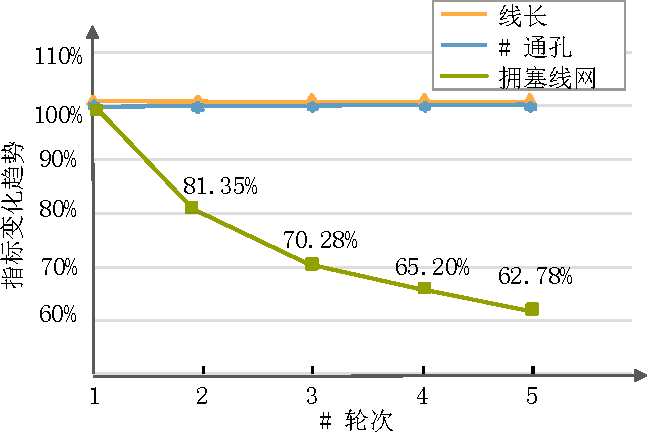
\includegraphics[width=0.86\textwidth]{image/chap03/指标变化趋势.pdf}
    \caption{迭代轮次下线长、通孔数与拥塞线网数量的归一化变化趋势}
    \label{fig:chap3-iter-overflow-placeholder}
\end{figure}

\subsection{拥塞疏解能力分析}

为进一步评估方法在全局尺度上的拥塞疏解能力，本文统计了各测试用例在整个版图所有布线格点上的溢出方差，并与CUGR2和DGR进行对比。该指标可反映拥塞分布的离散程度：若存在少量极端高拥塞区域，方差通常会明显增大；反之，方差较小意味着拥塞在空间上更均匀、极端热点更少。

\begin{table}[!htbp]
    \centering
    \caption{全版图布线格点溢出方差对比}
    \label{tab:chap3-overflow-variance}
    \small
    \setlength{\tabcolsep}{4.5pt}
    \renewcommand{\arraystretch}{1.05}
    \resizebox{0.70\textwidth}{!}{
        \begin{tabular}{l c c c}
            \hline
            测试用例 & CUGR2 & DGR & 本文方法\\
            \hline
            \texttt{ispd18\_test1} & \textbf{0.000000} & \textbf{0.000000} & \textbf{0.000000} \\
            \texttt{ispd18\_test2} & \textbf{0.000000} & \textbf{0.000000} & \textbf{0.000000} \\
            \texttt{ispd18\_test3} & \textbf{0.000033} & \textbf{0.000033} & \textbf{0.000033} \\
            \texttt{ispd18\_test4} & 0.000965 & 0.000343 & \textbf{0.000341} \\
            \texttt{ispd18\_test5} & 0.000330 & \textbf{0.000295} & \textbf{0.000295} \\
            \texttt{ispd18\_test6} & 0.000726 & 0.000403 & \textbf{0.000356} \\
            \texttt{ispd18\_test7} & 0.033941 & 0.008068 & \textbf{0.000178} \\
            \texttt{ispd18\_test8} & 0.033596 & 0.008540 & \textbf{0.000207} \\
            \texttt{ispd18\_test9} & 0.001612 & 0.000294 & \textbf{0.000283} \\
            \texttt{ispd18\_test10} & \textbf{0.001813} & 0.020782 & 0.008104 \\
            \texttt{ispd19\_test1} & \textbf{0.000000} & \textbf{0.000000} & \textbf{0.000000} \\
            \texttt{ispd19\_test2} & 0.000223 & 0.000067 & \textbf{0.000054} \\
            \texttt{ispd19\_test3} & 0.001121 & \textbf{0.001097} & \textbf{0.001097} \\
            \texttt{ispd19\_test4} & 0.977506 & 1.469525 & \textbf{0.677628} \\
            \texttt{ispd19\_test5} & 0.064924 & 0.054439 & \textbf{0.052443} \\
            \texttt{ispd19\_test6} & 0.040914 & 0.004348 & \textbf{0.000328} \\
            \texttt{ispd19\_test7} & \textbf{0.005015} & 0.017147 & 0.005351 \\
            \texttt{ispd19\_test8} & 0.003515 & 0.000051 & \textbf{0.000036} \\
            \texttt{ispd19\_test9} & 0.000057 & 0.000039 & \textbf{0.000025} \\
            \texttt{ispd19\_test10} & 0.001415 & \textbf{0.000492} & 0.000551 \\
            \texttt{ispd18\_test5\_metal5} & 0.046650 & 0.035846 & \textbf{0.030995} \\
            \texttt{ispd18\_test8\_metal5} & 0.086847 & 0.091664 & \textbf{0.063235} \\
            \texttt{ispd18\_test10\_metal5} & \textbf{0.079482} & 0.650815 & 0.517773 \\
            \texttt{ispd19\_test7\_metal5} & \textbf{0.067776} & 0.145810 & 0.116442 \\
            \texttt{ispd19\_test8\_metal5} & 0.112746 & 0.112154 & \textbf{0.102457} \\
            \texttt{ispd19\_test9\_metal5} & \textbf{0.085597} & 0.095206 & 0.087988 \\
            \texttt{ariane133\_51} & 0.001042 & 0.000018 & \textbf{0.000009} \\
            \texttt{ariane133\_68} & 0.006327 & 0.000260 & \textbf{0.000079} \\
            \texttt{bsg\_chip} & 0.060302 & 0.025314 & \textbf{0.017464} \\
            \texttt{mempool\_tile} & 0.002731 & 0.001423 & \textbf{0.000713} \\
            \texttt{nvdla} & 0.129507 & 0.062775 & \textbf{0.011053} \\
            \hline
        \end{tabular}
    }
\end{table}

由表\ref{tab:chap3-overflow-variance}可见，本文按逐case比较并将最小方差加粗标注。在31个测试用例中，本文方法在25个用例上达到最小方差（含并列最小），明显多于CUGR2的9个和DGR的7个。与此同时，本文方法的最大方差为0.677628（\texttt{ispd19\_test4}），低于CUGR2的0.977506和DGR的1.469525，说明本文方法在全局上更能抑制极端拥塞热点，整体拥塞化解能力更强。

进一步地，为讨论极限拥塞场景下的热点化解能力，本文统计了每个测试用例中拥塞最严重的前千分之一布线格点的方差，并绘制对比柱状图，如图\ref{fig:chap3-top001-hotspot-variance}所示。需要注意的是，为了有效可视化，对于三种方法方差均为0的用例（\texttt{ispd18\_test1}、\texttt{ispd18\_test2}、\texttt{ispd19\_test1}），由于不存在可区分的热点波动，图中不再绘制。对其余有效测试用例，按逐case归一化：将该case三种方法中的最大方差设为100\%，其余方法按相对比例换算。

\begin{figure}[!htbp]
    \centering
    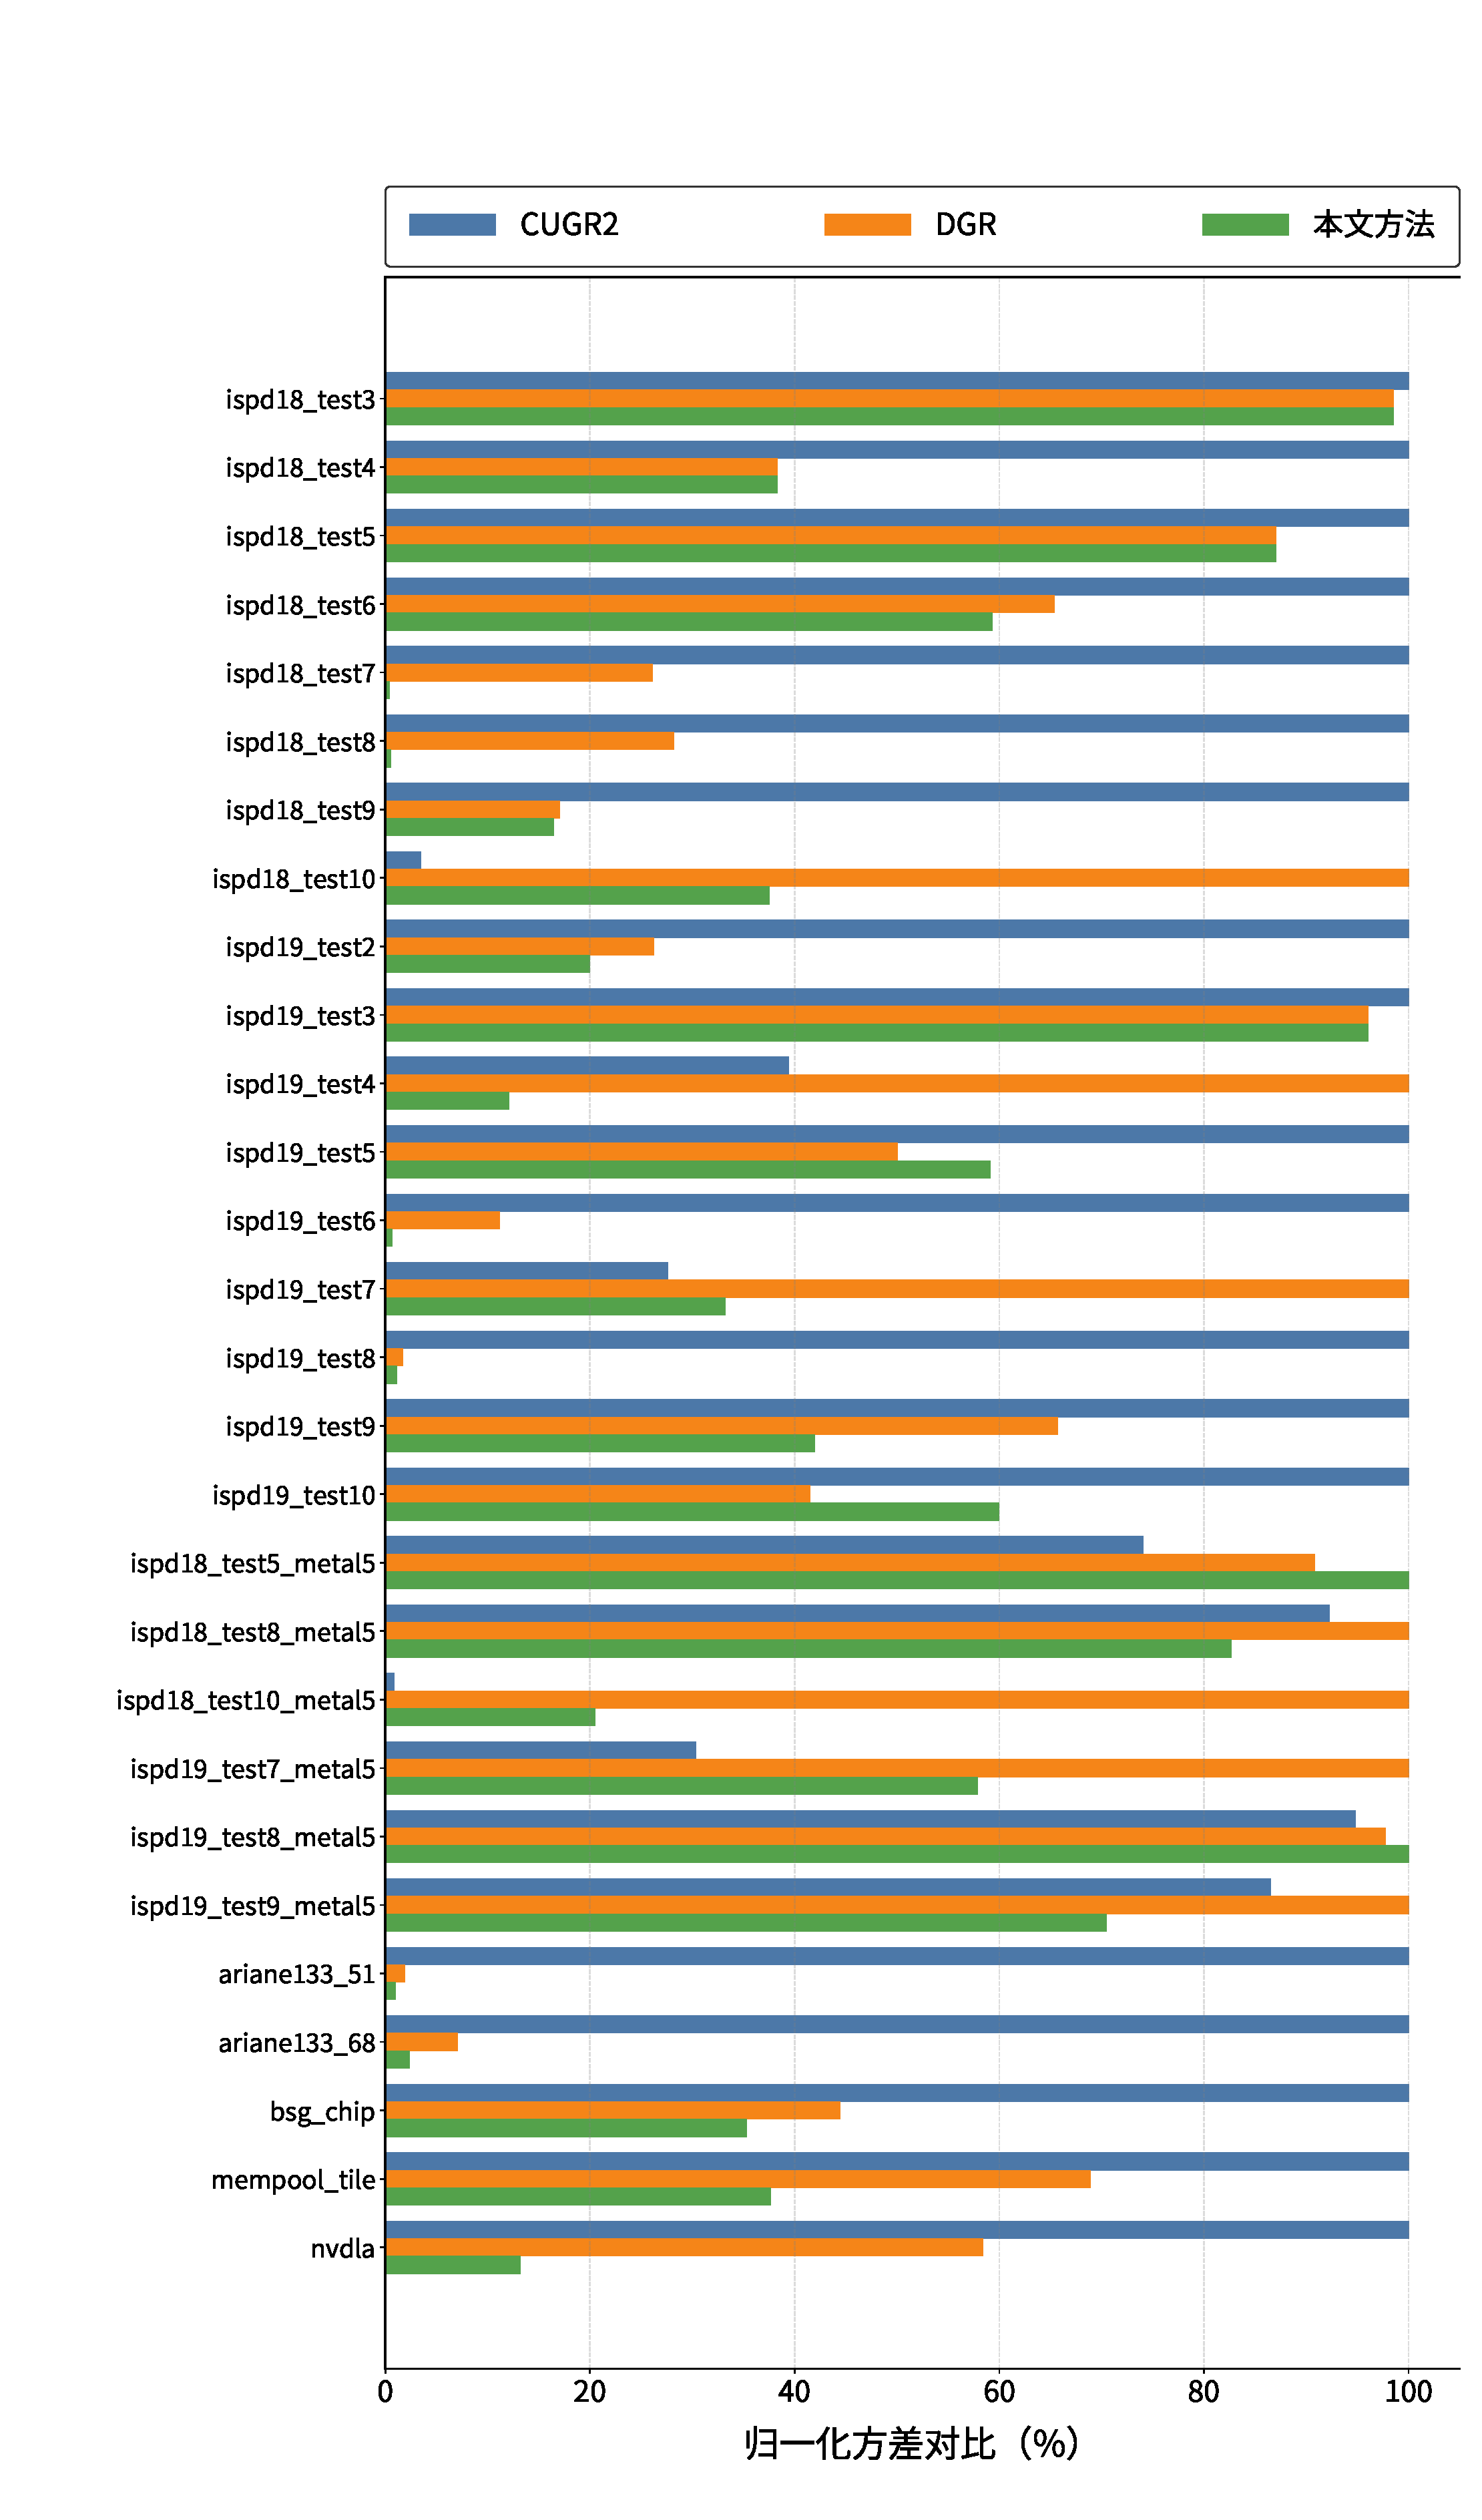
\includegraphics[width=0.96\textwidth]{image/chap03/top001_hotspot_variance_normalized_barh.pdf}
    \caption{前千分之一严重拥塞格点方差归一化对比}
    \label{fig:chap3-top001-hotspot-variance}
\end{figure}

从图\ref{fig:chap3-top001-hotspot-variance}可见，在大量高难度用例上，本文方法对应柱长普遍更短，说明在统一归一化基准下其热点方差更低，即极端拥塞区域的波动被更有效地压制。该结果与前文全版图方差结论相互印证，进一步表明本文方法不仅改善整体拥塞分布，也能更有针对性地缓解高风险拥塞热点。

% \subsection{结果讨论与局限性}

% 综合实验可得两点结论。第一，动态拥塞感知初始布线在拥塞主导场景中的收益更显著，说明前期候选质量对后续流程具有放大效应。第二，动态更新与动态缩减形成了互补机制，在保证质量收益的同时控制了额外计算成本。

% 同时也应看到局限性：
% \begin{enumerate}
%     \item 当初始拥塞较轻时，动态更新带来的相对收益可能下降；
%     \item 在极端高密度场景下，候选树数目与模板数目的增长仍会增加显存压力；
%     \item 现有流程主要针对初始布线阶段，和后续迷宫布线的深度协同仍有进一步研究空间。
% \end{enumerate}

% 这些局限性为后续工作提供了明确方向：一是探索更细粒度的自适应候选扩展策略；二是强化跨阶段信息传递机制，在初始布线与后续细化布线之间建立更紧密的反馈闭环。

% % \subsection{参数敏感性分析}

% % 为评估流程对关键超参数的敏感性，本文进一步考察以下参数：
% % \begin{enumerate}
% %     \item 迭代上限 $R_{max}$；
% %     \item 概率阈值 $\theta$（用于离散化判定）；
% %     \item 三项损失权重 $\lambda_{wl},\lambda_{via},\lambda_{of}$；
% %     \item 温度退火速率与学习率衰减系数。
% % \end{enumerate}

% % 实验观察表明：
% % \begin{enumerate}
% %     \item 当 $R_{max}$ 过小时，拥塞难以充分下降；过大时边际收益下降明显；
% %     \item 较高的 $\theta$ 有利于提高决策确定性，但过高可能导致早期有效候选被误抑制；
% %     \item 提高 $\lambda_{of}$ 可显著改善拥塞，但若过高会带来线长与通孔指标波动；
% %     \item 温度退火与学习率衰减需要协同设置，过快退火可能引起过早收敛。
% % \end{enumerate}

% % 总体上，参数敏感性结果支持本文采用的默认参数区间，即在拥塞改善和综合代价之间取得稳健折中。

% % \begin{table}[!htbp]
% %     \centering
% %     \caption{关键参数敏感性结果（占位）}
% %     \label{tab:chap3-param-sens-placeholder}
% %     \fbox{\parbox{0.90\textwidth}{
% %             表格占位：后续可填入不同参数配置下Overflow、Wirelength、Via、Runtime变化比例。
% %         }}
% % \end{table}

% \subsection{典型案例分析：拥塞热点的演化过程}

% 除总体指标外，本文对典型高拥塞设计进行可视化分析。结果显示，初始轮次的拥塞热点通常集中在宏单元边界通道与跨区连接密集带；随着动态更新树与动态缩减策略推进，热点区域面积逐步收缩，高溢出边数量显著下降。

% 从路径层面看，RSMT候选在早期提供了较短主干，而拥塞感知候选在热点区域提供了替代绕行方案。训练过程通过概率分化逐步完成候选切换，最终形成主干短、局部绕的折中布局。该现象验证了双候选设计的互补性，也解释了为何本文方法在不显著牺牲线长的情况下可降低拥塞。

% \begin{figure}[!htbp]
%     \centering
%     \fbox{\parbox{0.92\textwidth}{
%             \centering
%             插图占位\\
%             建议插入内容：典型案例拥塞热力图（迭代前/中/后对比）\\
%             对比内容：热点面积、峰值溢出、拥塞带连通性变化
%         }}
%     \caption{典型案例拥塞热力图演化（占位）}
%     \label{fig:chap3-case-heatmap-placeholder}
% \end{figure}

% \begin{figure}[!htbp]
%     \centering
%     \fbox{\parbox{0.92\textwidth}{
%             \centering
%             插图占位\\
%             建议插入内容：典型线网拓扑演化对比（RSMT候选 vs 更新后候选）\\
%             对比内容：路径穿越拥塞区情况、边移动前后局部资源占用
%         }}
%     \caption{典型线网拓扑演化示意（占位）}
%     \label{fig:chap3-case-topology-placeholder}
% \end{figure}

% \subsection{工程可迁移性讨论}

% 从工程部署角度，本文流程具有以下可迁移性特征：
% \begin{enumerate}
%     \item 与现有全局布线框架接口清晰，可作为初始布线增强模块接入；
%     \item 树森林构建、可微训练、动态更新与动态缩减可分别模块化实现，便于逐步上线；
%     \item 并行化实现对硬件平台有较好适配性，可根据资源规模选择不同批处理配置。
% \end{enumerate}

% 同时，迁移过程中需重点关注两点：其一，不同工业设计的约束分布差异可能影响默认参数鲁棒性；其二，若后续阶段布线策略变化较大，需同步调整初始布线的代价建模权重，以保持跨阶段目标一致性。

% \subsection{有效性威胁与复现实践建议}

% 为保证实验结论的可靠性，本节从内部有效性、外部有效性与复现实践三个维度进行讨论。

% 第一，内部有效性方面，核心风险在于参数耦合导致的表面提升。例如，当 $\lambda_{of}$ 过高时，溢出指标可能显著下降，但同时带来线长或通孔恶化。如果仅报告单一指标，容易高估方法收益。为缓解该风险，建议始终以多指标联合报告，并在消融实验中给出参数变化下的整体趋势，而非单点最优结果。

% 第二，外部有效性方面，测试基准分布与真实工业设计可能存在偏差。公开基准在规模、宏单元密度、时序压力与工艺约束上不一定覆盖所有工业场景，因此在公开基准有效不等价于在所有工业场景同样有效。本文建议在后续工程验证中补充不同类型设计，包括高扇出控制逻辑、存储器密集型设计和跨层互连密集型设计，以更全面评估方法泛化能力。

% 第三，复现实践方面，本文建议采用固定配置 + 逐项变更原则开展实验复现。具体做法为：先在固定随机种子、固定批处理策略、固定学习率计划下复现实验基线，再逐项改变动态更新频率、缩减阈值、候选生成规则，记录各项指标变化。该流程可有效避免多因素同时变更导致的归因不清问题。

% 此外，为提高后续实验可追溯性，建议将每次运行的关键元数据统一记录，包括代码版本、编译选项、硬件型号、驱动版本、参数配置文件哈希值与日志摘要。通过建立标准化实验登记表，可以显著降低后续对比分析的成本。

% \begin{table}[!htbp]
%     \centering
%     \caption{实验复现实践清单（占位）}
%     \label{tab:chap3-repro-checklist-placeholder}
%     \fbox{\parbox{0.90\textwidth}{
%             表格占位：后续可填入检查项-记录内容-是否必选三列，\\
%             建议包含代码版本、参数文件、随机种子、硬件环境、日志归档路径等条目。
%         }}
% \end{table}

% 从论文写作角度看，上述有效性与复现讨论具有两方面价值：一是进一步明确本章结论的适用边界，避免结论外推过度；二是为后续章节及未来工作提供可直接执行的实验规范。这种结果 + 边界 + 复现的三位一体表达，有助于提升章节论证完整性与学术可信度。

\section{本章小结}
\label{sec:chap3-summary}

本章围绕拥塞感知初始布线工作流，系统介绍了从候选树森林构建、可微解析建模，再到树森林动态更新与规模缩减策略，并详细介绍了技术实现细节。与DGR相比，本文方法通过更新拥塞线网候选 + 缩减非拥塞线网训练集合的闭环策略，使优化过程具备持续反馈能力，能够在线长、通孔数指标维持稳定的前提下显著降低溢出相关指标。

% 从方法层面看，双候选树森林为线长导向与拥塞导向提供了统一决策空间；两层概率建模将离散选择问题转化为可微优化问题；动态机制在多轮训练中持续重塑候选空间并抑制无效计算。从工程层面看，数据级并行与线网级并行协同提升了大规模场景下的求解吞吐，使该流程具备较好的可扩展性。

实验结果表明，本文流程在拥塞相关指标上取得了稳定改进，并在可控计算开销下实现了质量与效率的协同增益。%以上结论为后续章节的进一步分析与拓展提供了方法基础。
